%
% $Id: blank.tex,v 2.0 2010-01-05 18:50:50+09 kobayasi Exp $
%
% Mar 21, 2001:  Revision Control Started!!
%
\documentclass[11pt]{jreport}
\usepackage{newcent}             % PDFへの変換後の品質を高める
\usepackage[dvipdfmx]{graphicx}
\usepackage{color}
\definecolor{purple}{rgb}{0.6,0,0.4}
\definecolor{brown}{cmyk}{0,0.81,1,0.60}
\definecolor{gray}{rgb}{0.4,0.4,0.4}
\definecolor{darkblue}{rgb}{0.0,0.0,0.6}
\definecolor{cyan}{rgb}{0.0,0.6,0.6}
\usepackage{listings, jlisting}
\renewcommand{\lstlistingname}{ソースコード}
\lstdefinestyle{MyJava} % JavaとXML,2つの言語を使いたかったので.style=MyJavaとかで使い分け
{
language=Java, % lstlisting内の言語の指定
numbers=left, % 行番号を左端に表示する
breaklines = true, % 行が長くなってしまった場合の改行を行う
basicstyle={\small}, % 標準の書式設定
identifierstyle={\small}, % 識別子のスタイル
keywordstyle={\small\bfseries\color{purple}}, % キーワードのスタイル
commentstyle={\small\itshape\color{gray}}, % コメントのスタイル
stringstyle={\small\ttfamily\color{brown}}, % 文字列のスタイル
frame=single, % 枠のスタイル
tabsize=2, % タブ幅
showstringspaces=false, % 空白を可視化するか
}
\lstdefinelanguage{XML} % XMLはあまり充実してないってさー
{
    morestring=[b]",
    morestring=[s]{>}{<},
    morecomment=[s]{<?}{?>},
    stringstyle=\color{brown},
    identifierstyle=\color{darkblue},
    keywordstyle=\color{cyan},
    morekeywords={xmlns,version,type}% list your attributes here
}
\lstdefinestyle{MyXML} % JavaとXM(ry
{
language=XML,
numbers=left,
breaklines=true,
basicstyle={\small},
identifierstyle={\small\color{darkblue}},
keywordstyle={\small\bfseries\color{cyan}},
commentstyle={\small\itshape\color{gray}},
stringstyle={\small\ttfamily\color{brown}},
frame=single,
tabsize=2,
showstringspaces=false,
}

\renewcommand{\slash}{/}
\graphicspath{{./Screenshots/}, {./Graphs/},{./Figures/}} %Where the app screenshots folder is located
\usepackage{otf} % OpenType Font utfなどにしか無いような文字を利用する
\usepackage{longtable} % ページをまたぐ表の作成

\usepackage{sotsuron}               % 卒業研究概要の場合

\setlength\textfloatsep{0pt}

\title{\bfseries スマートフォンのモーションセンサを利用した\\個人認証アプリケーションの開発}
\author{情11-170 \UTF{9AD9}坂 賢佑}
\date{}
\renewcommand{\bibname}{参考文献,参考URL等}

\begin{document}
\maketitle

\tableofcontents
\listoffigures

\chapter*{はじめに}
スマートフォンが徐々に普及しつつある現在,スマートフォンの個人認証方法は画面上に表示されるソフトウェアキーボードのテンキーを用いたパスコード認証が大部分を占めている.
しかし,この認証方法は画面ロックを解除するたびに画面に表示されたソフトウェアキーボードを目で見て指でタッチして操作する必要があるため,ユーザにとって煩雑な作業である.
また,あらかじめ決められた文字種の中から一つずつ選択したものを元にパスコードを構築していくという性質上,パターン数が限られ自由度が限定されてしまう.

そこで,本研究ではパスコード認証が抱える認証の煩雑さを解消し,かつ自由度が高くより直感的に個人認証を行えるアプリケーションを開発する.
このアプリケーションには,一般的なスマートフォンに搭載されている加速度センサとジャイロセンサを用いる.

% ^^^^^^^^^^^^^^^^^^^^^^^^^^^^^^^^^^^^^^^^^^^^^^^^^^^^^^^^^^
% ^^^^^^^^^^^^^^^^^^^^^^^^^^^^^^^^^^^^^^^^^^^^^^^^^^^^^^^^^^
%               使用するセンサについて
% vvvvvvvvvvvvvvvvvvvvvvvvvvvvvvvvvvvvvvvvvvvvvvvvvvvvvvvvvv
% vvvvvvvvvvvvvvvvvvvvvvvvvvvvvvvvvvvvvvvvvvvvvvvvvvvvvvvvvv
\chapter{使用するセンサについて}
本アプリケーションには2種類のモーションセンサを利用する.

    \section{加速度センサ}
    加速度センサとは,X軸,Y軸,Z軸の基準軸に対して直線運動の加速度をそれぞれ検出し,値として取り出すことのできるセンサである.
    ここでいう加速度とは端末における単位時間あたりの速度の変化率のことを指し,図\ref{sensor}における直線で示した矢印の方向が正の値,逆が負の値をとる.

    \section{ジャイロセンサ}
    ジャイロセンサとは,X軸,Y軸,Z軸の基準軸に対して回転運動の角速度をそれぞれ検出し,値として取り出すことのできるセンサである.
    ここでいう角速度とは端末における単位時間あたりの回転角のことを指し,図\ref{sensor}における橙色で示した回転の方向が正の値,逆が負の値をとる.

    % センサのイメージ図
    \begin{figure}[hbtp]
      \begin{center}
        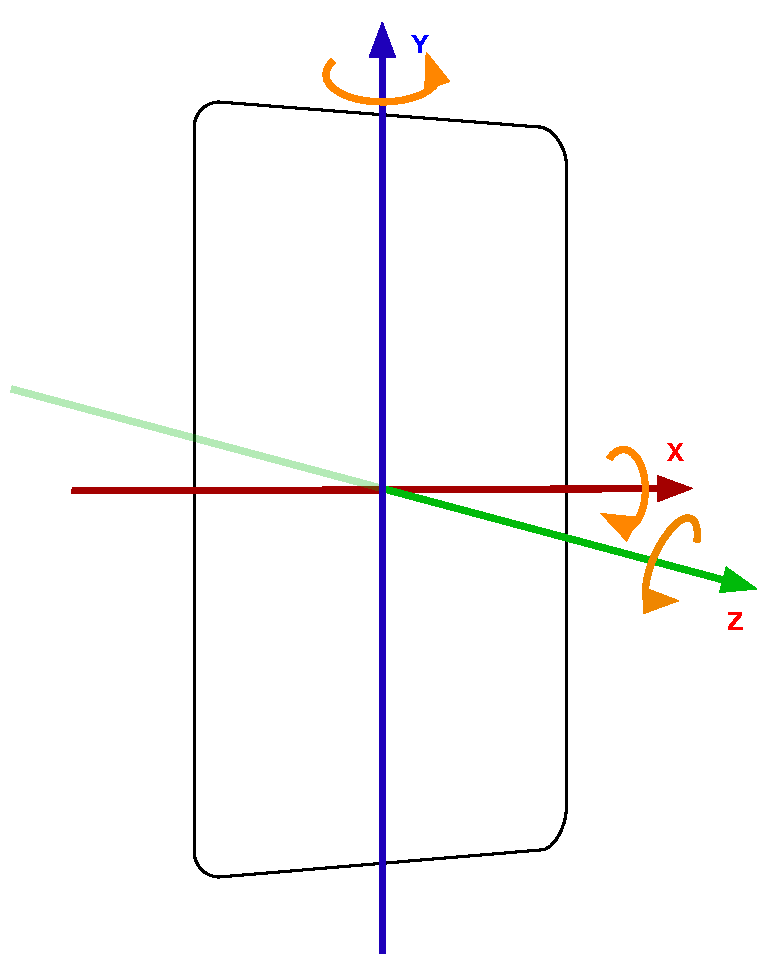
\includegraphics[width=7cm, bb=0 0 373 469]{SmartphoneSensor.pdf}
        \caption{モーションセンサの座標系イメージ}
        \label{sensor}
      \end{center}
    \end{figure}

% ^^^^^^^^^^^^^^^^^^^^^^^^^^^^^^^^^^^^^^^^^^^^^^^^^^^^^^^^^^
% ^^^^^^^^^^^^^^^^^^^^^^^^^^^^^^^^^^^^^^^^^^^^^^^^^^^^^^^^^^
%                       先行研究
% vvvvvvvvvvvvvvvvvvvvvvvvvvvvvvvvvvvvvvvvvvvvvvvvvvvvvvvvvv
% vvvvvvvvvvvvvvvvvvvvvvvvvvvvvvvvvvvvvvvvvvvvvvvvvvvvvvvvvv
\chapter{先行研究}
    \section{坂本の研究}
    坂本の研究\cite{sakamoto}では,ユーザが入力したモーションの数値化に加速度センサを用い,あらかじめ保存しておいた複数のジェスチャパターンのデータと認証時に入力したデータをパターンマッチング方式のアルゴリズムを用いて比較することで個人認証を行った.

    しかし,このプログラムは扱うジェスチャによって認証率が高いものと低いものに二分化する傾向が見られるという問題点があった.

    \section{兎澤の研究}
    兎澤の研究\cite{tozawa}では,モーションの数値化に加速度センサとジャイロセンサを用い,認証システムの中核に相関関数を用いたシステムを開発し,ユーザに3回入力させたモーションの平均値データと認証時に入力したデータの類似性を調べることで個人認証を行った.
    これにより,坂本の研究で指摘されていた成功率の二分化や立体的な動きへの対応を可能にし,モーションの対応幅を広げることができた.

    しかし,全体的な認証成功率が低く,特に手首のスナップを用いるような動きの小さいモーションに対して認証率が特に低く出るなど,対応できるモーションに限りがあるという問題点が指摘されていた.

% ^^^^^^^^^^^^^^^^^^^^^^^^^^^^^^^^^^^^^^^^^^^^^^^^^^^^^^^^^^
% ^^^^^^^^^^^^^^^^^^^^^^^^^^^^^^^^^^^^^^^^^^^^^^^^^^^^^^^^^^
%                    本研究のシステム
% vvvvvvvvvvvvvvvvvvvvvvvvvvvvvvvvvvvvvvvvvvvvvvvvvvvvvvvvvv
% vvvvvvvvvvvvvvvvvvvvvvvvvvvvvvvvvvvvvvvvvvvvvvvvvvvvvvvvvv
\chapter{本研究のシステム}
    \section{本研究の概要}
    本研究では兎澤の研究で挙げられていた,全体的な認証成功率の低さや対応できるモーションに限りがあるという点を改善することを目標とする.
    具体的には,より幅広いモーション,特に手首のスナップを用いるような比較的動きの小さいモーションに対しての個人認証の全体的な認証成功率の向上を目指し,実用レベルに近いアプリケーションの開発を行う.

    \section{システムの概要}
    本研究では,先行研究をもとにAndroidデバイス上で動作するアプリケーションとしてシステムを構築した.
    システムの動作フローを図\ref{flow}に示す.

    % システム動作フロー図
    \begin{figure}[btp]
        \begin{center}
            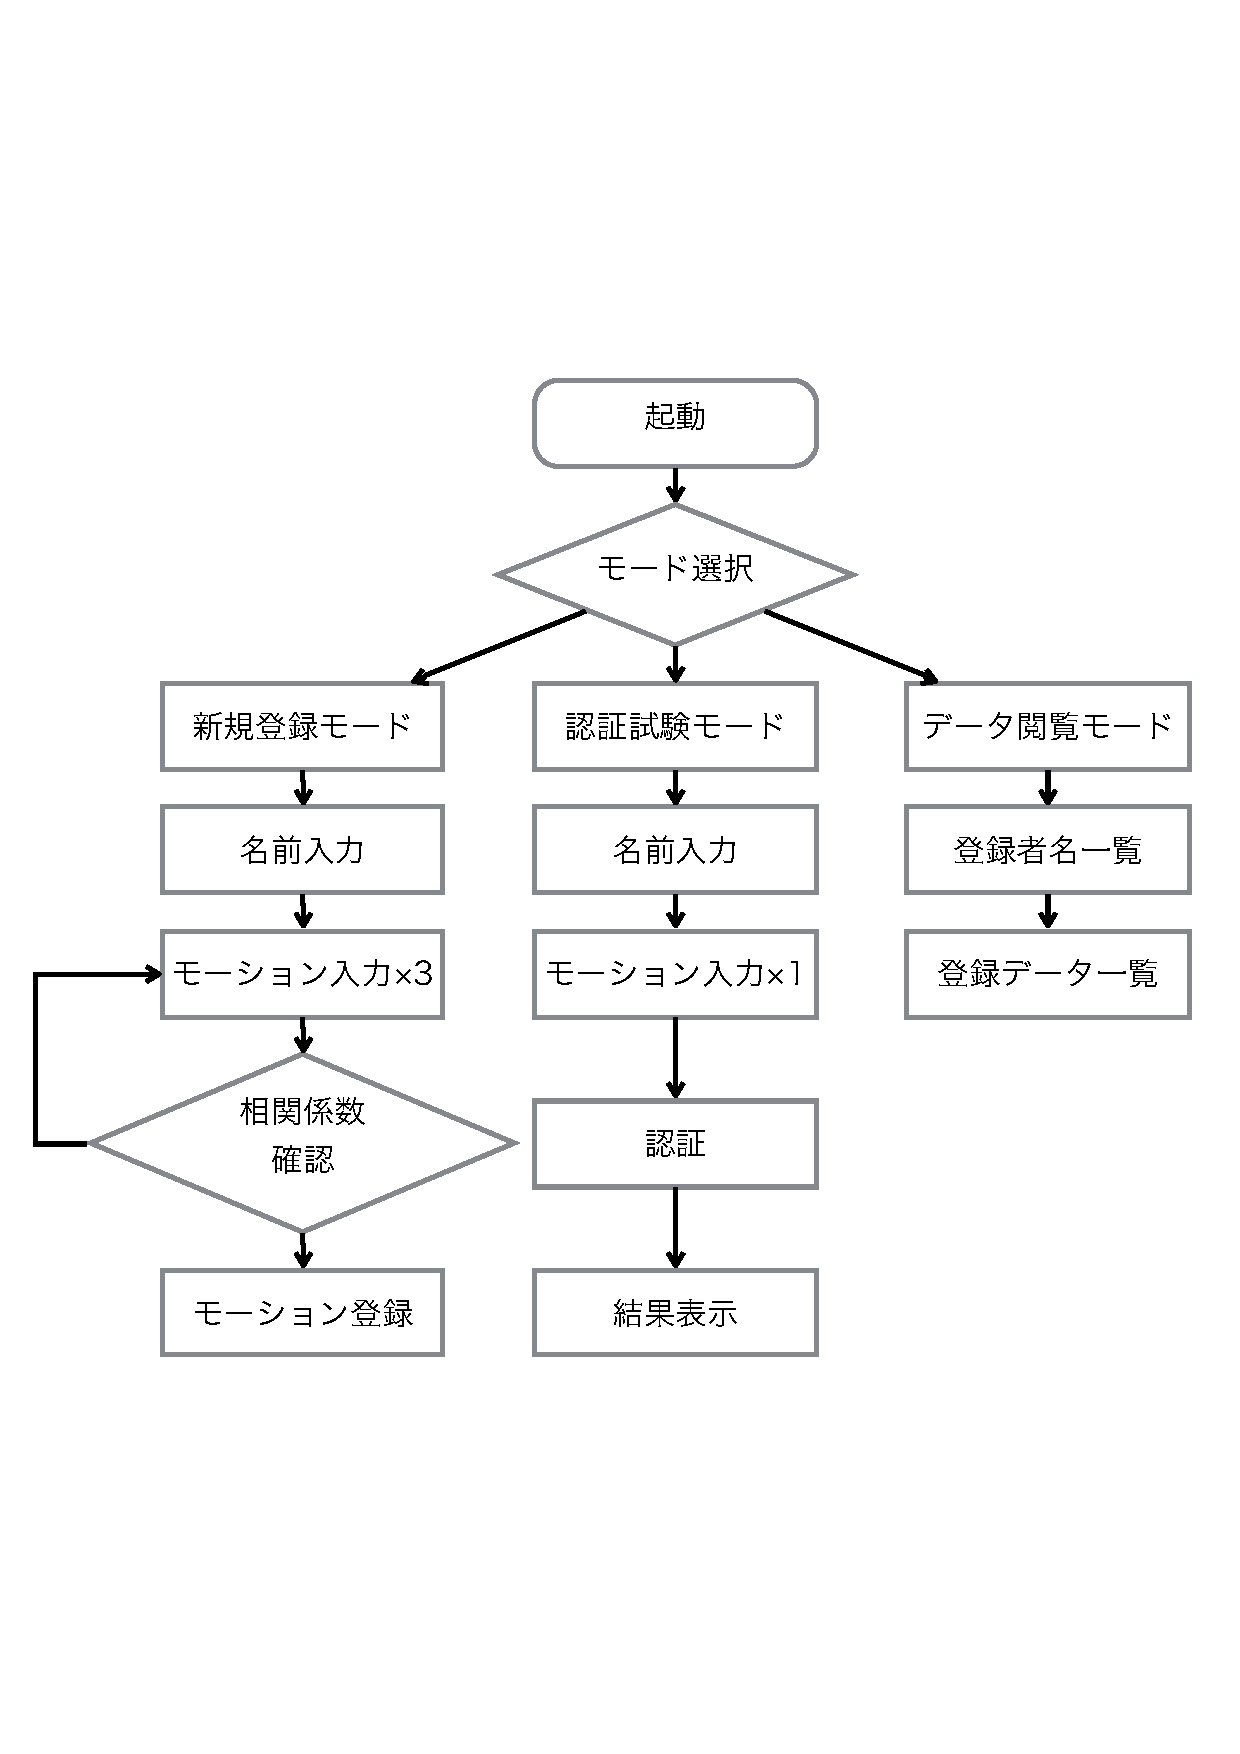
\includegraphics[width=9cm, bb=0 183 594 670]{Flow.pdf}
            \caption{システム動作フロー図}
            \label{flow}
        \end{center}
    \end{figure}

    アプリケーション起動時は,図\ref{start}のような起動画面が表示される.
    ここでStartボタンを押すことで,図\ref{selectMode}のようなモード選択ダイアログが表示される.

    ユーザはまず,新規登録モードにおいて個人認証に用いる鍵情報となるモーションをユーザ名と共に登録する.
    このモードでは,ユーザに登録したい同一のモーションを3回入力してもらう.
    入力された3回のモーションが同一のモーションであると確認できた場合に,この平均値をユーザのモーションデータとして登録する.

    認証試験モードでは,事前に新規登録モードにおいてモーションデータを登録したユーザ名を入力し,該当ユーザが登録されていると確認できた場合にのみユーザにモーションを1回入力してもらう.
    入力されたモーションデータと指定したユーザ名で登録されたモーションデータとの相関を取ることで個人認証を行う.

    データ閲覧モードでは,新規登録モードにおいて登録したユーザ名およびモーションデータをリスト形式で閲覧することが出来る.

    % スタート画面スクリーンショット
    \begin{figure}[tbp]
        \begin{minipage}{0.5\hsize}
            \begin{center}
                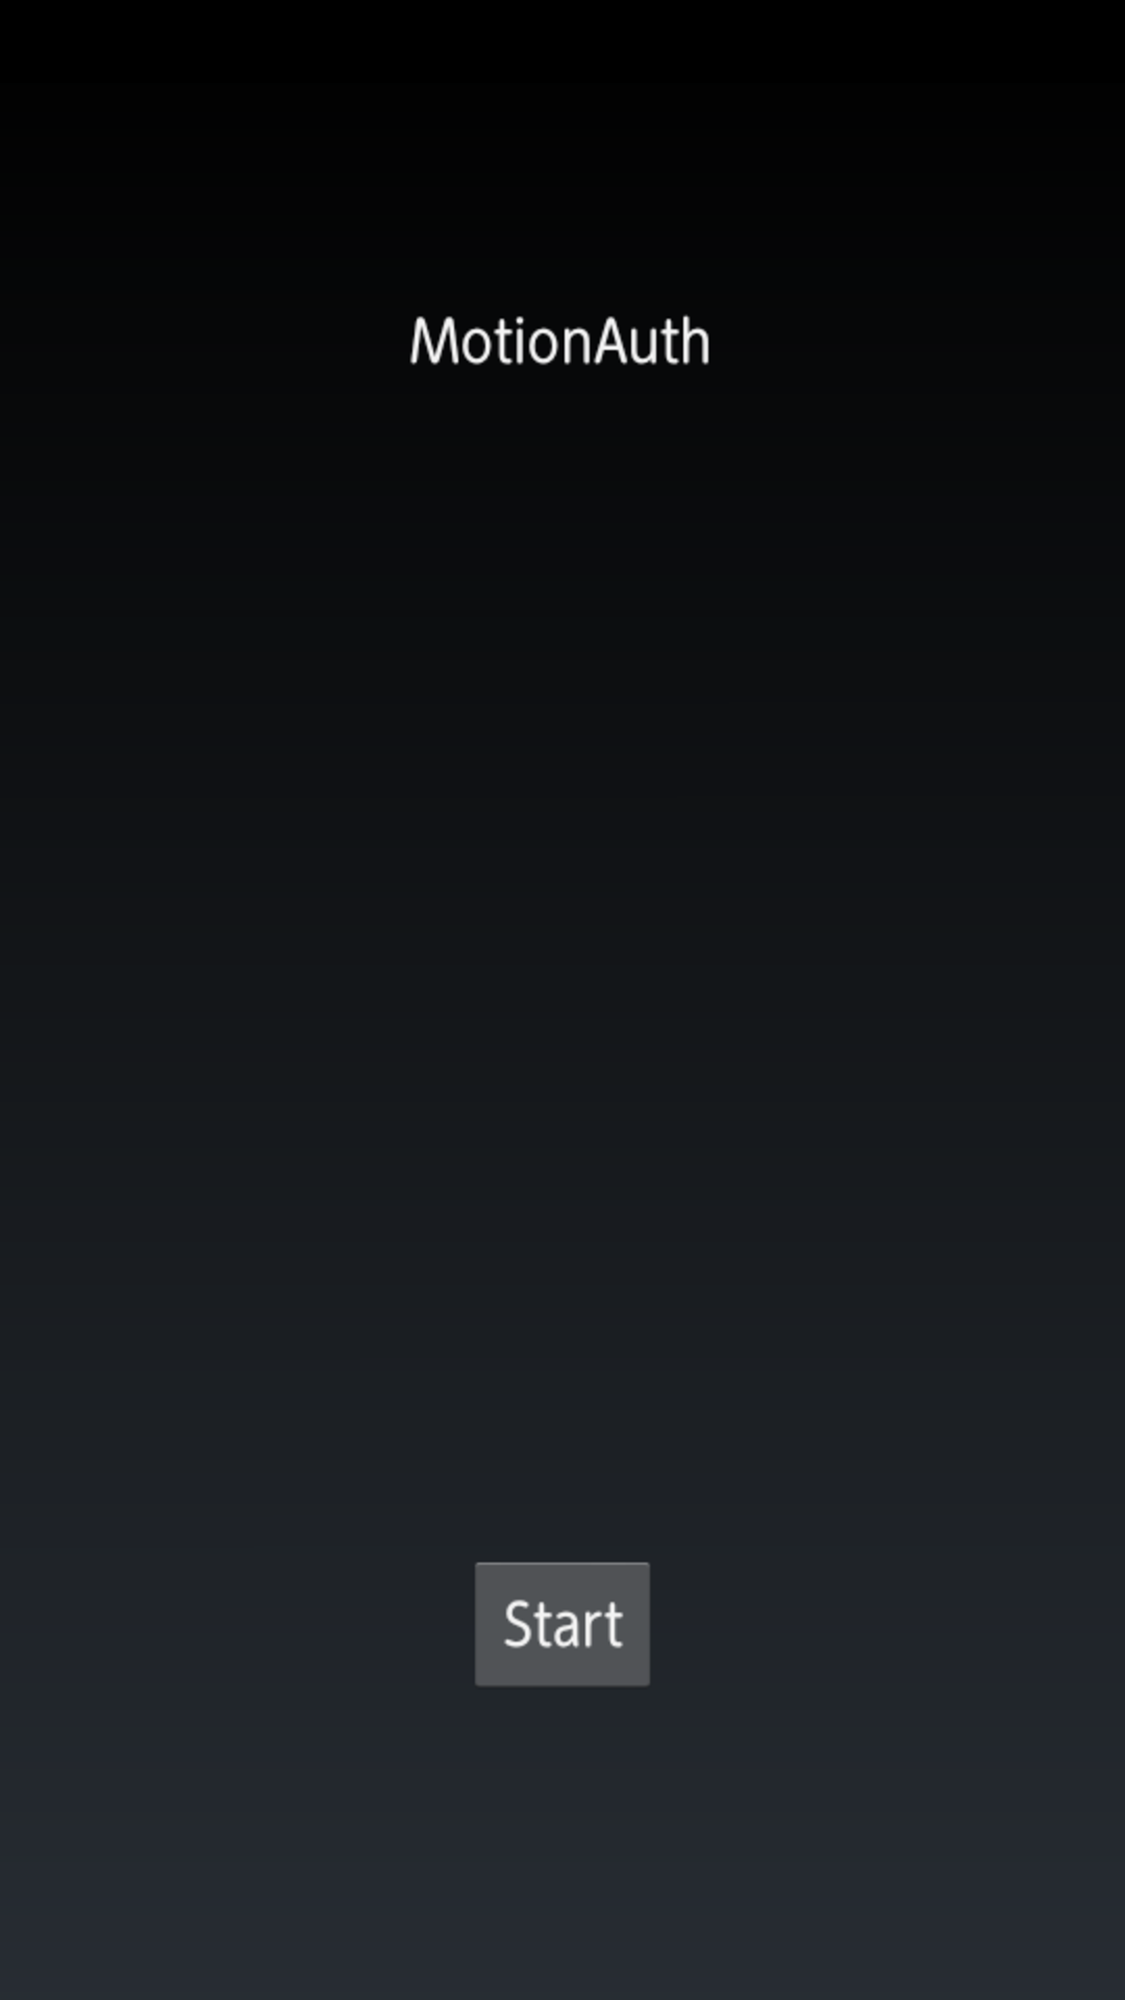
\includegraphics[width=5cm, bb=0 0 540 960]{Start.pdf}
            \end{center}
            \caption{スタート画面}
            \label{start}
        \end{minipage}
        \begin{minipage}{0.5\hsize}
            \begin{center}
                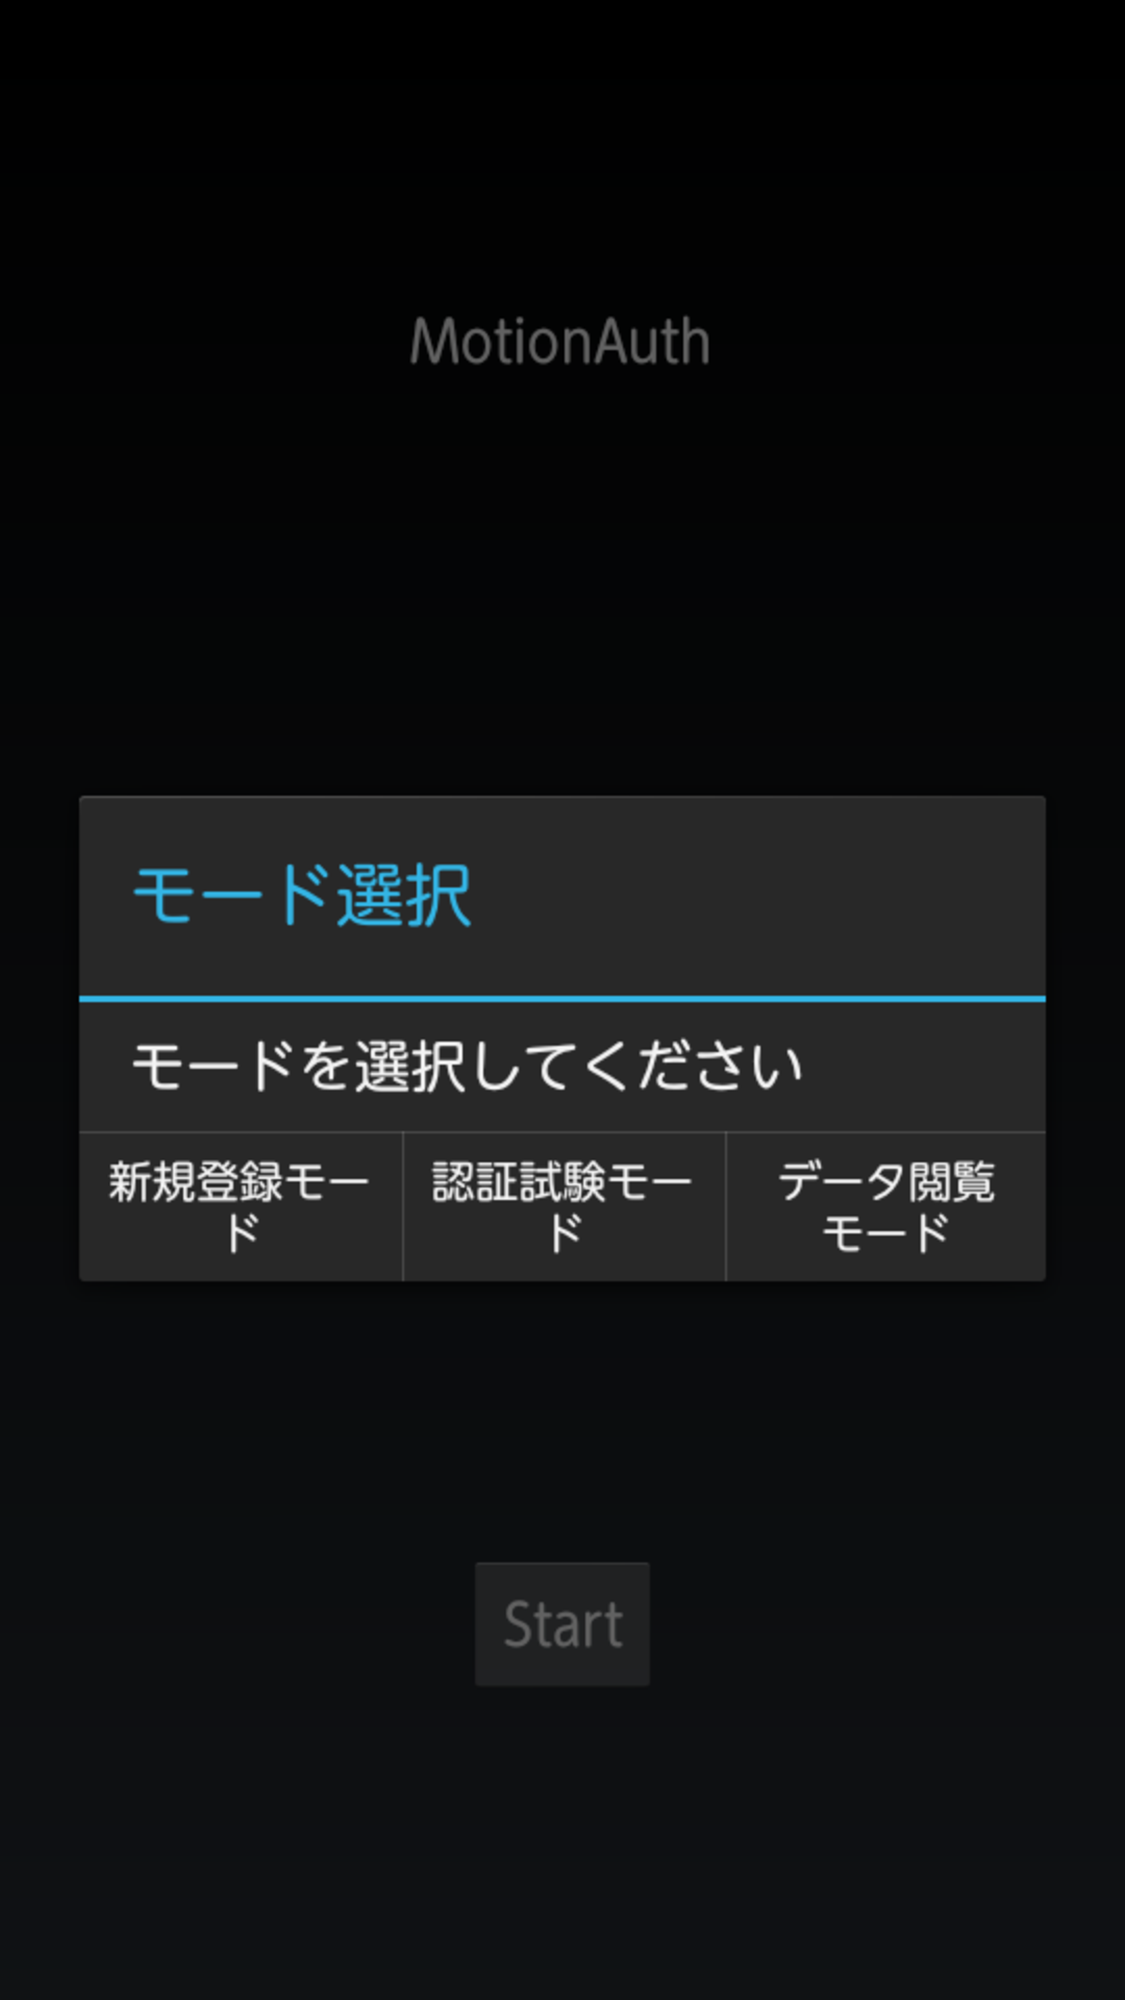
\includegraphics[width=5cm, bb=0 0 540 960]{ModeSelect.pdf}
            \end{center}
            \caption{モード選択ダイアログ}
            \label{selectMode}
        \end{minipage}
    \end{figure}

        % 各モードに対して,説明をもっと掘り下げる
% ^^^^^^^^^^^^^^^^^^^^^^^^^^^^^^^^^^^^^^^^^^^^^^^^^^^^^^^^^^
%                    新規登録モード
% vvvvvvvvvvvvvvvvvvvvvvvvvvvvvvvvvvvvvvvvvvvvvvvvvvvvvvvvvv
\newpage
        \subsection{新規登録モード}
        新規登録モードでは,まず図\ref{nameInput}の画面において登録したいユーザの名前を入力する.
        この画面においてOKボタンを押した際にテキストフィールドが空であれば,図\ref{nameInputError}のような通知を表示してユーザに名前の再入力を促す.
        テキストフィールドが空でなければ,次の図\ref{reg}の画面においてモーションの登録を行う.
        OKボタンを押した際の名前の入力値チェックを行うコードをソースコード\ref{regCheckInputNameSource}に示す.

        % ユーザ名入力画面
        \begin{figure}[tbhp]
            \begin{minipage}{0.33\hsize}
                \begin{center}
                    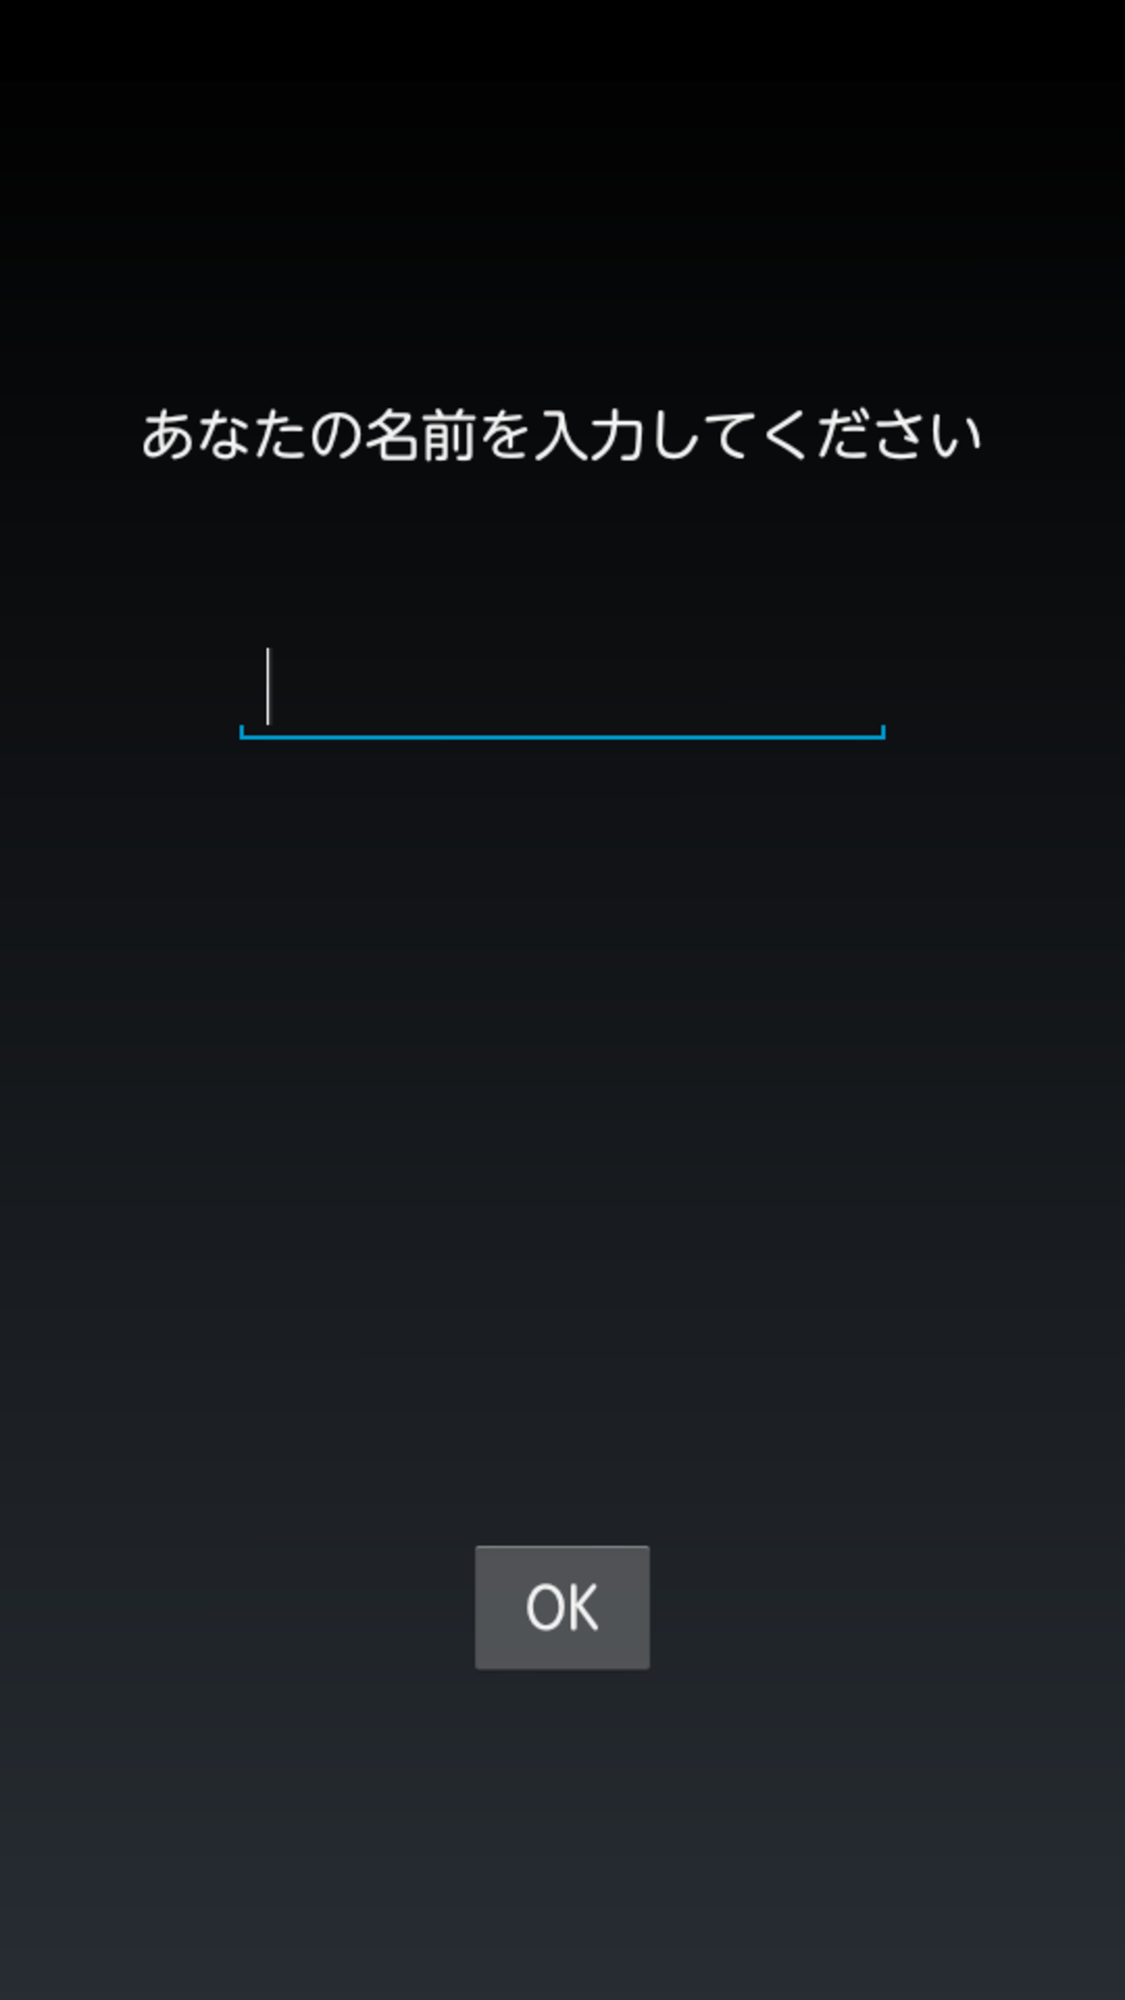
\includegraphics[width=5cm, bb=0 0 540 960]{NameInput.pdf}
                \end{center}
                \caption{ユーザ名入力画面}
                \label{nameInput}
            \end{minipage}
            \begin{minipage}{0.33\hsize}
                \begin{center}
                    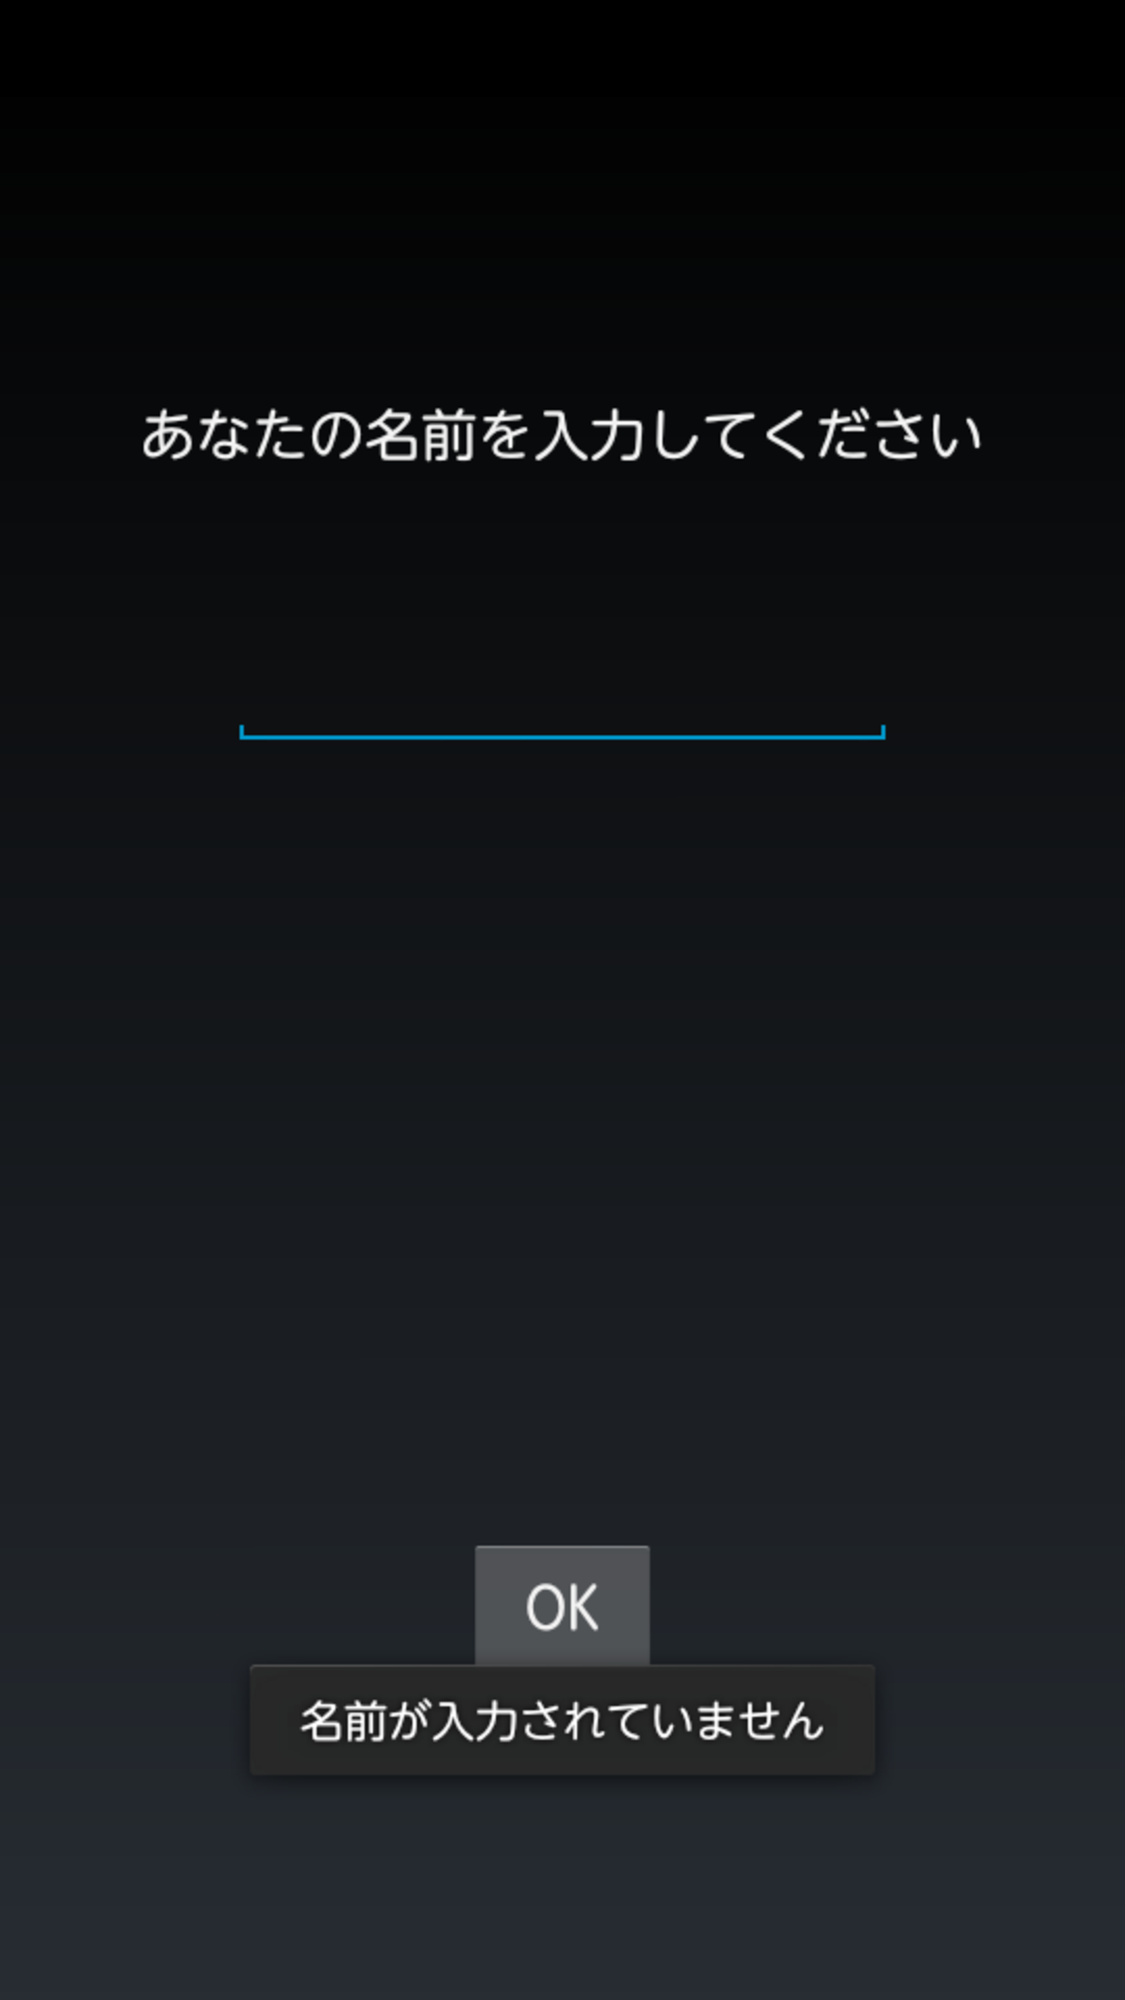
\includegraphics[width=5cm, bb=0 0 540 960]{NameInputError.pdf}
                \end{center}
                \caption{エラー通知}
                \label{nameInputError}
            \end{minipage}
            \begin{minipage}{0.33\hsize}
                \begin{center}
                    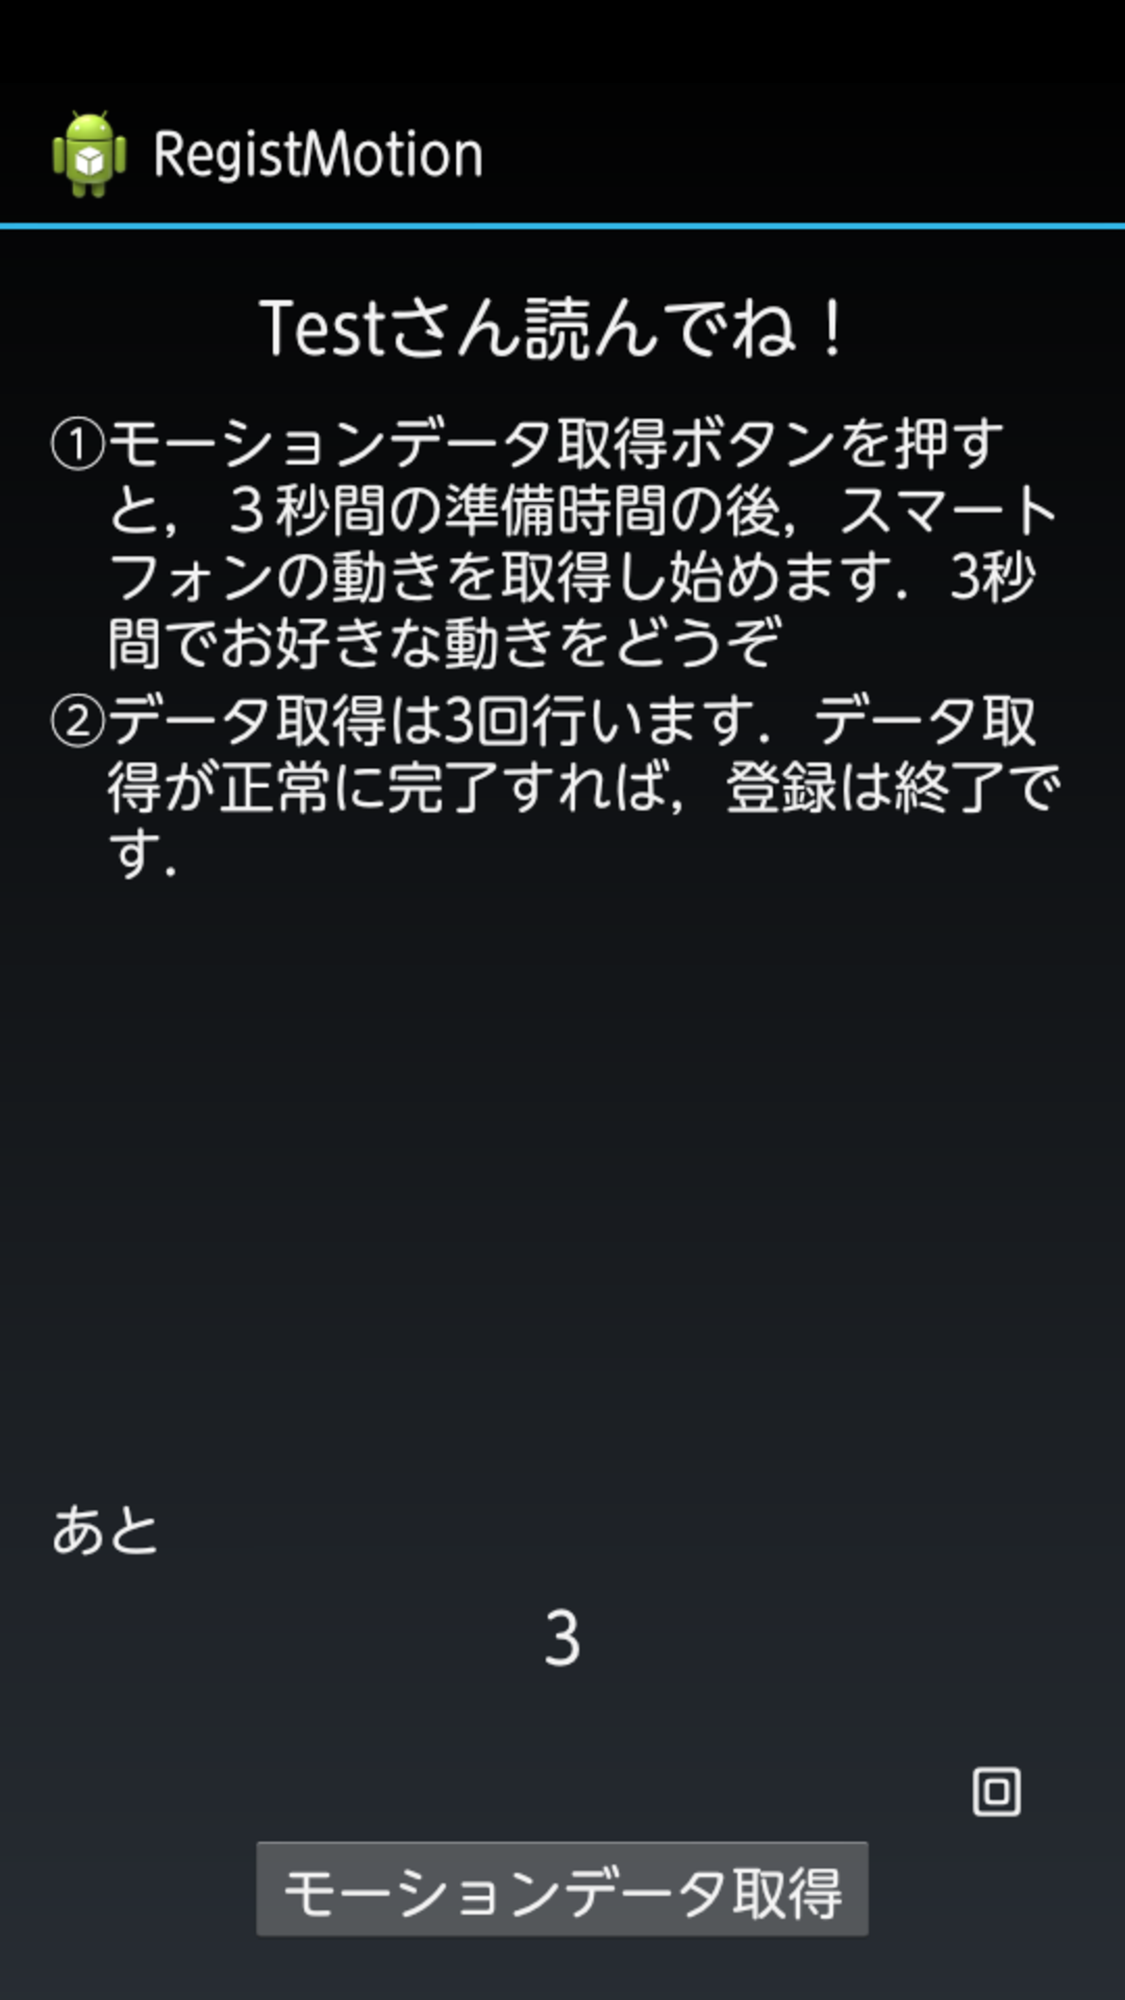
\includegraphics[width=5cm, bb=0 0 540 960]{Reg.pdf}
                \end{center}
                \caption{モーション登録画面}
                \label{reg}
            \end{minipage}
        \end{figure}

        \lstinputlisting[caption=入力値チェック, label=regCheckInputNameSource, style=MyJava]
        {Code\slash regCheckInputName}

        モーション登録画面においてモーションデータ取得ボタンを押すと,3秒間のインターバルを挟んだ後にモーションデータの取得を3秒間行う.
        この際,画面の下部にそれぞれの経過秒数を表示し,ヴァイブレーションにて1秒毎の時間経過を知らせるようにしている.

        モーションデータの取得は加速度データ,ジャイロデータそれぞれを0.03秒ごとにセンサから取得し,X・Y・Z軸のそれぞれから100個ずつ,計600個を1回分として取得する.

        モーションデータの取得が3回行われると図\ref{regProgress}のような計算処理待ちダイアログが表示され,データの加工が行われる.
        あらかじめ増幅器の閾値を設定しておき,取得したデータの振れ幅が閾値より1回でも小さい場合はモーションの動きが小さいと判断し,全てのデータに振れ幅の増幅処理を行う.
        次にフーリエ変換を用いたローパスフィルタ処理によって,モーション取得時の手の細かなブレなどから生じうるデータに対する影響を取り除く.
        ローパスフィルタ処理が終われば,取得したデータが同一のものであるかの確認を行う.
        同一のものであると確認されなければ,モーションデータの取り直しを行う.
        同一のものであると確認されれば,モーション取得時に生じうる時間的なズレを必要に応じて修正する.
        ズレ修正の処理が終われば3回分のデータ間の相関係数を算出し,相関が認められた場合は図\ref{regSuccess}のような登録完了ダイアログを表示する.
        このダイアログのOKボタンを押すことで,取得した3回分のデータの平均値データと増幅量を保存し,起動画面に移動する.
        相関が認められなかった場合は,図\ref{regFail}のような登録失敗ダイアログを表示する.
        このダイアログのOKボタンを押すことでプログラム内部のモーションデータ取得カウンタが初期化され,モーションデータの取り直しをさせる.

        % モーション登録画面
        \begin{figure}[bthp]
            \begin{minipage}{0.33\hsize}
                \begin{center}
                    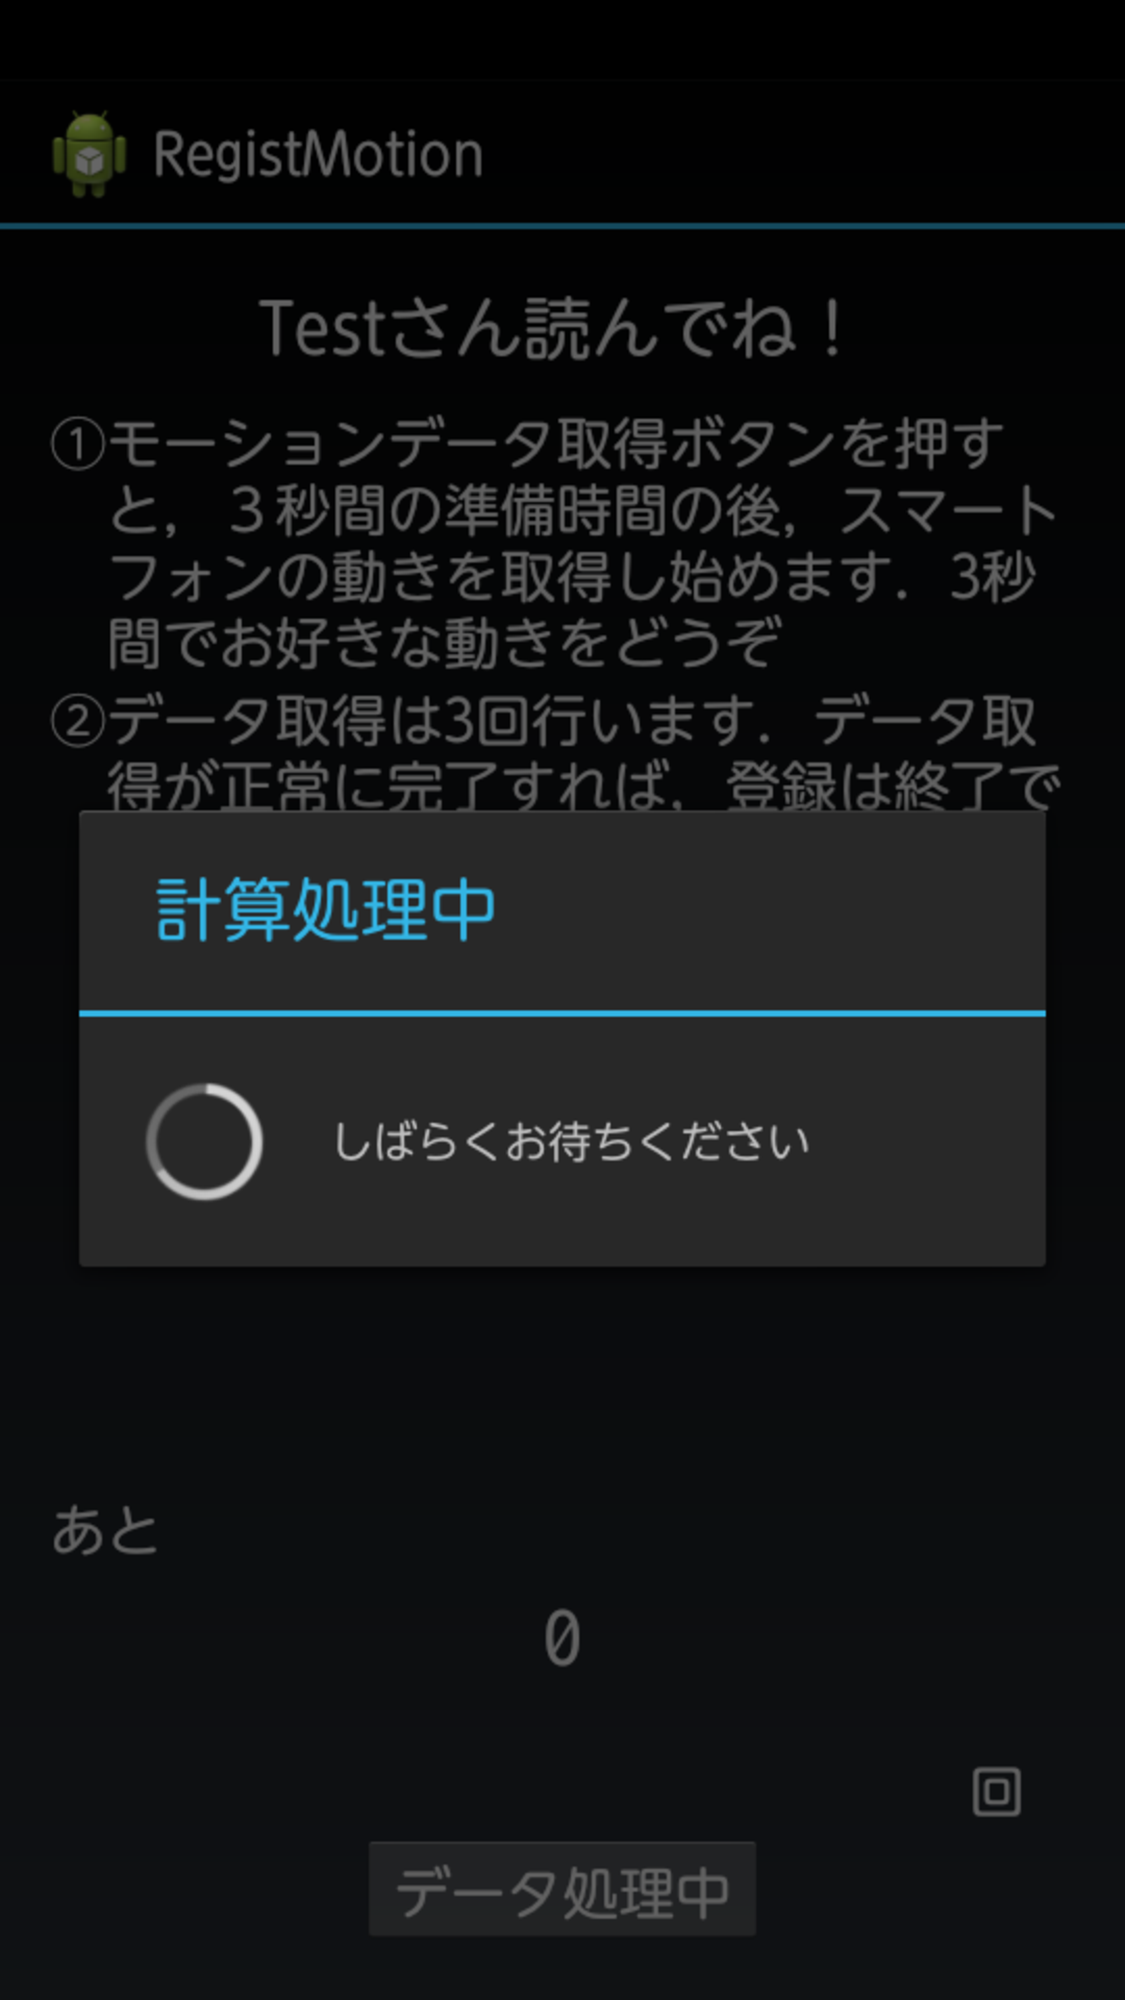
\includegraphics[width=5cm, bb=0 0 540 960]{RegProgress.pdf}
                \end{center}
                \caption{処理待ちダイアログ}
                \label{regProgress}
            \end{minipage}
            \begin{minipage}{0.33\hsize}
                \begin{center}
                    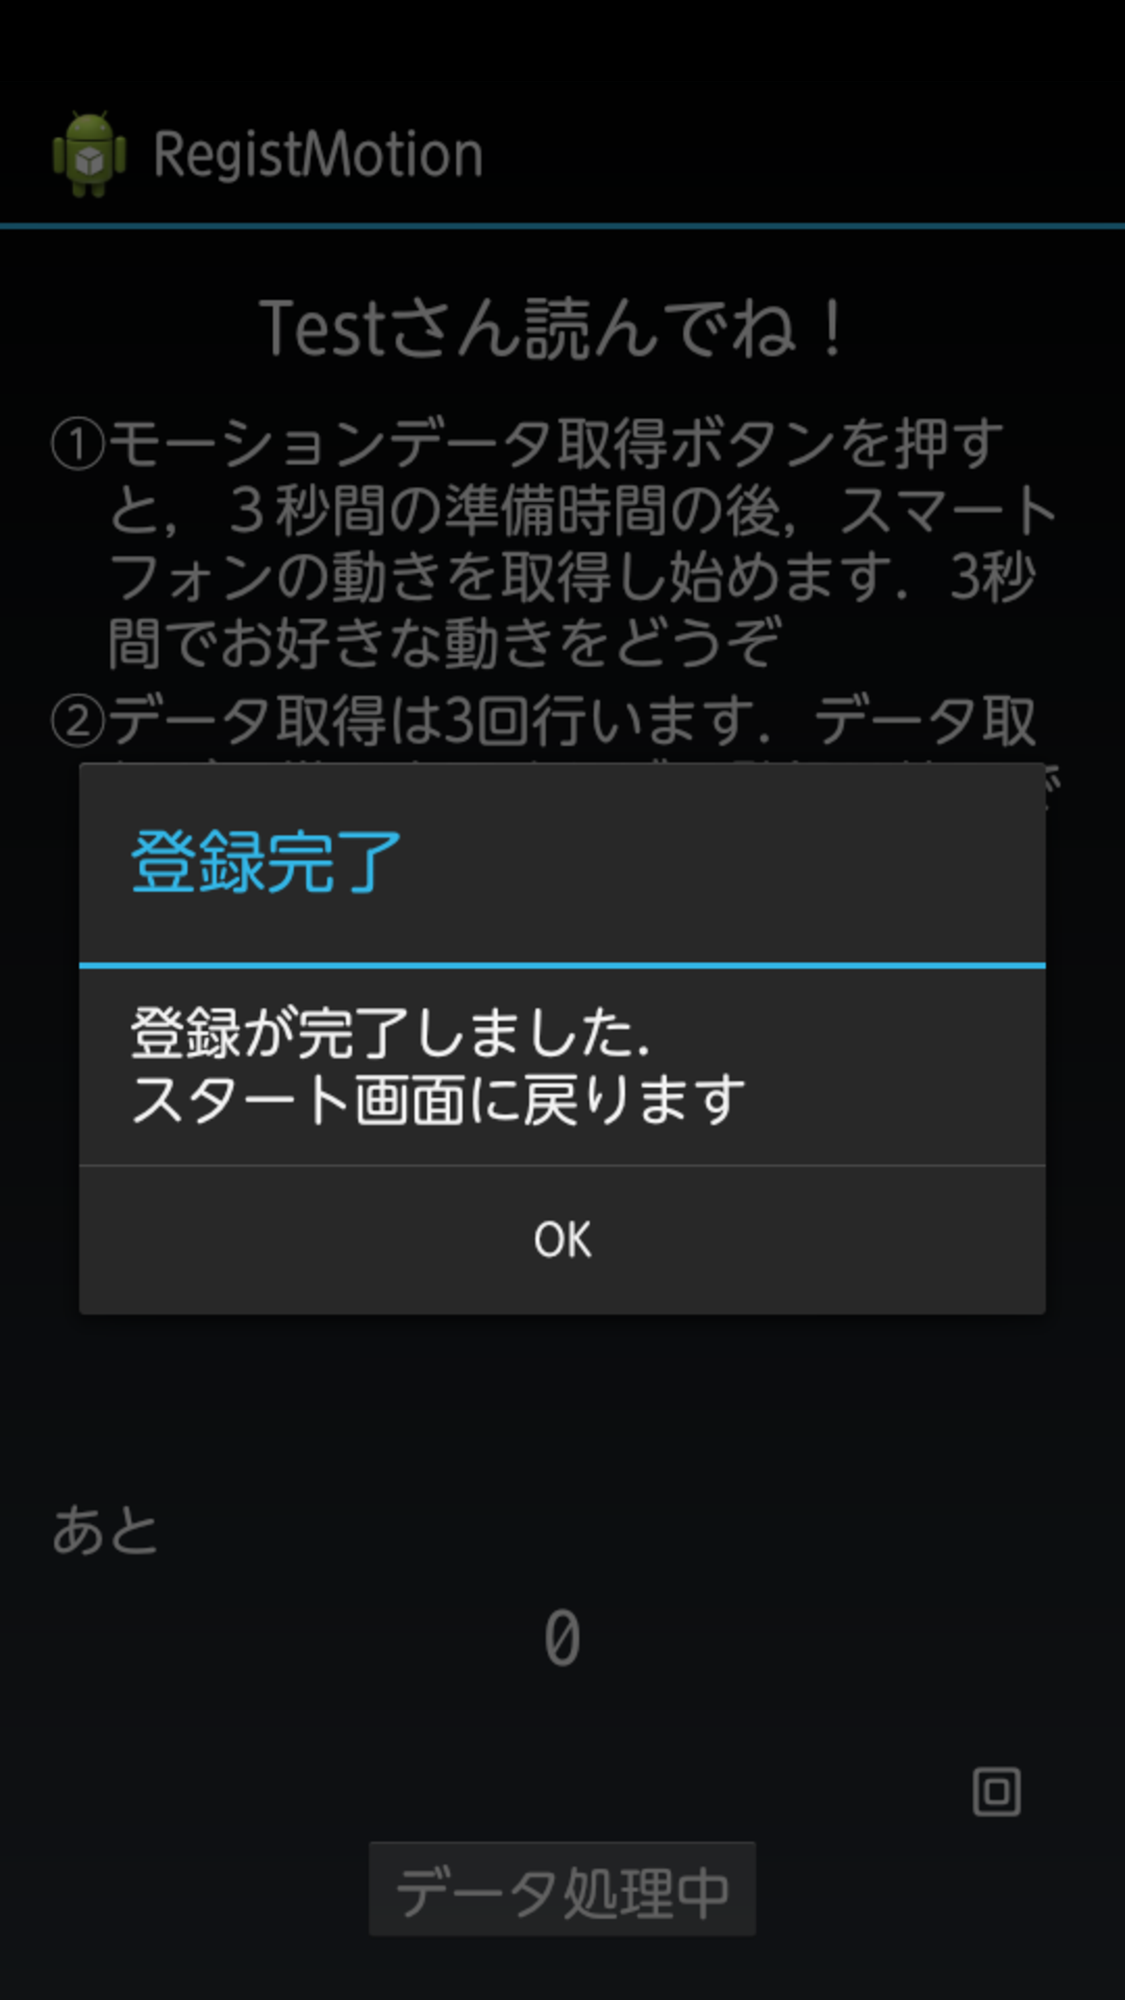
\includegraphics[width=5cm, bb=0 0 540 960]{RegSuccess.pdf}
                \end{center}
                \caption{登録完了ダイアログ}
                \label{regSuccess}
            \end{minipage}
            \begin{minipage}{0.33\hsize}
                \begin{center}
                    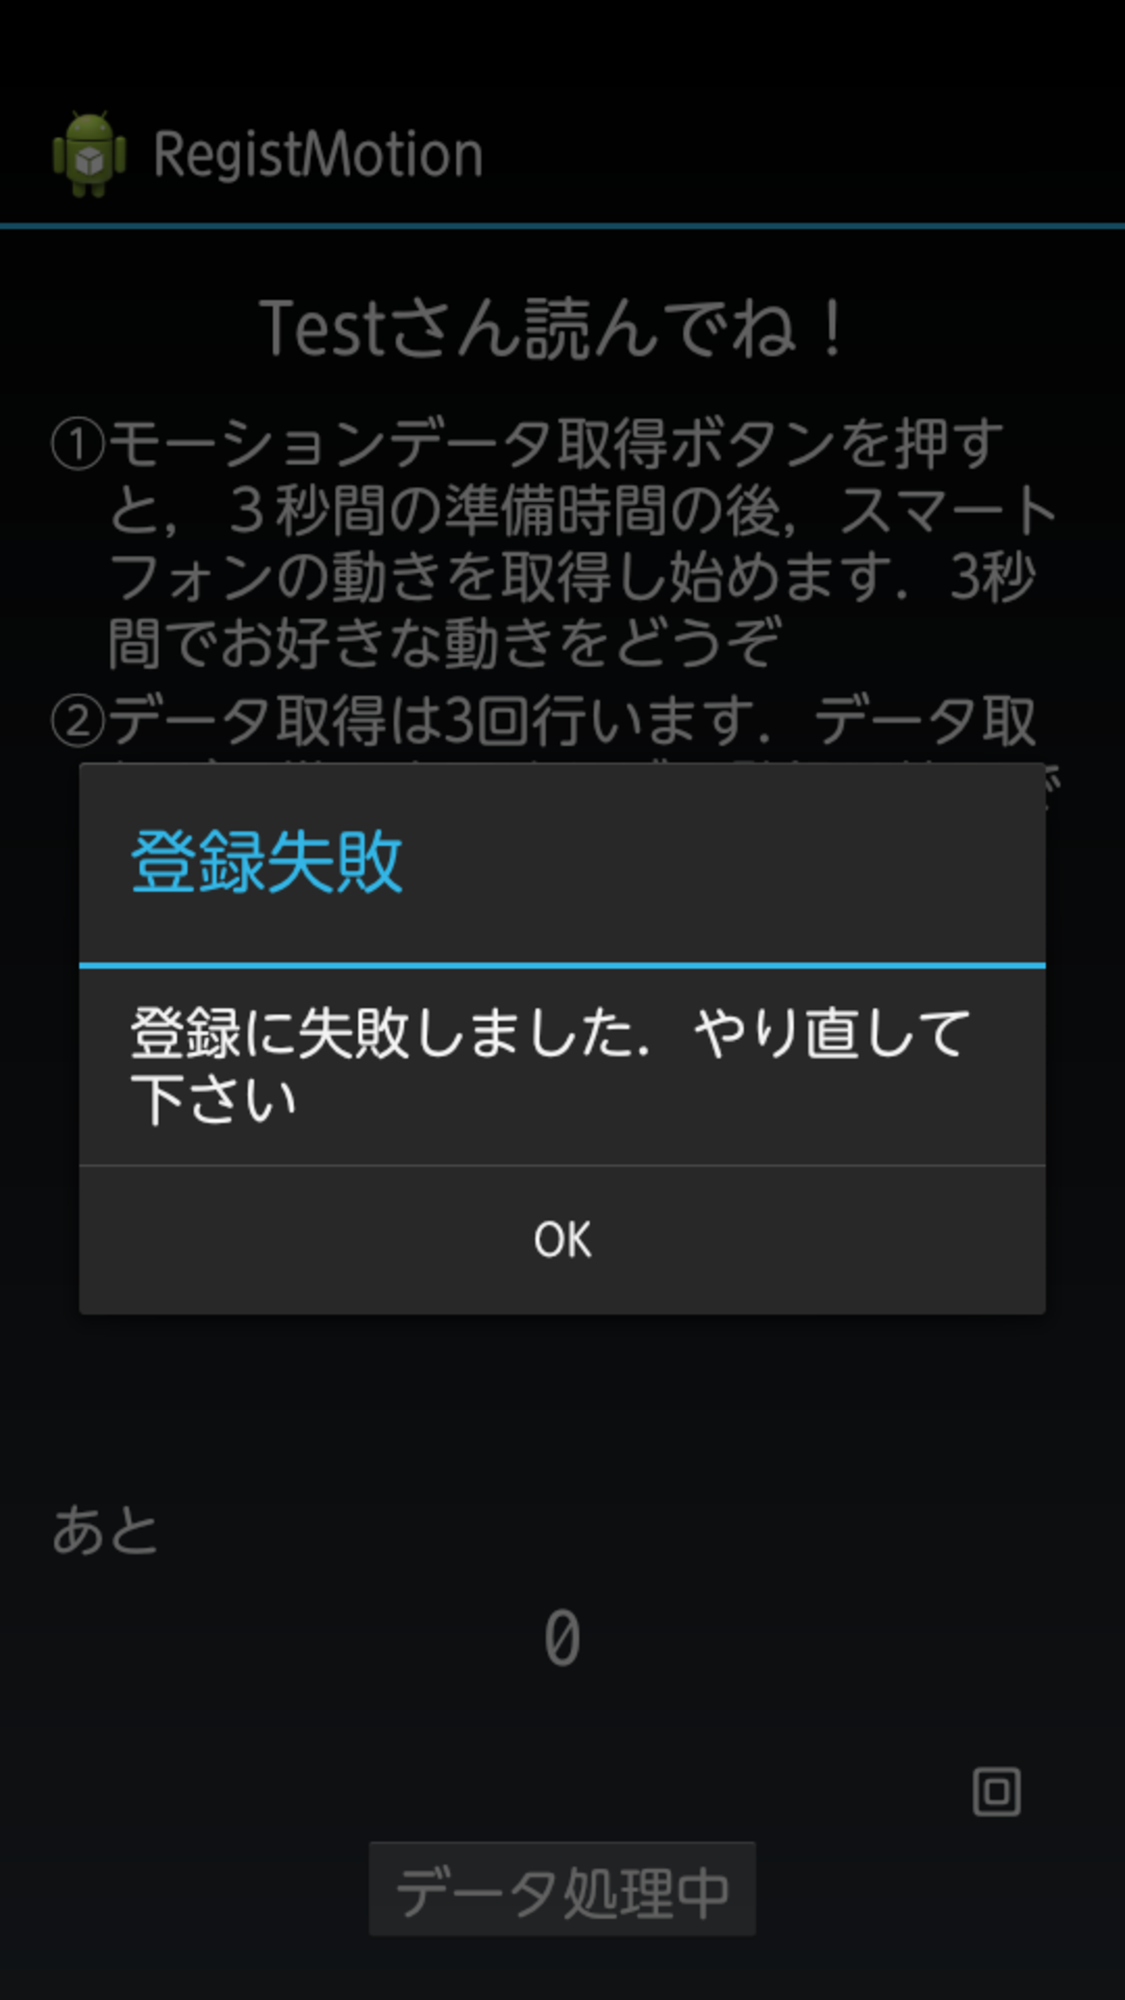
\includegraphics[width=5cm, bb=0 0 540 960]{RegFail.pdf}
                \end{center}
                \caption{登録失敗ダイアログ}
                \label{regFail}
            \end{minipage}
        \end{figure}

% ^^^^^^^^^^^^^^^^^^^^^^^^^^^^^^^^^^^^^^^^^^^^^^^^^^^^^^^^^^
%                    認証試験モード
% vvvvvvvvvvvvvvvvvvvvvvvvvvvvvvvvvvvvvvvvvvvvvvvvvvvvvvvvvv
        \subsection{認証試験モード}
        認証試験モードでは,まず図\ref{authNameInput}の画面において新規登録モードであらかじめ登録されたユーザ名を入力する.
        指定されたユーザ名で既にモーションの登録がなされていることが確認できた場合にのみ,図\ref{auth}の画面で個人認証を行う.
        モーションの登録がなされていなかった場合,図\ref{authNameInputError}のようなダイアログを表示する.
        指定されたユーザ名で既にモーションの登録がなされているかを確認するコードをソースコード\ref{authCheckInputNameSource}に示す.

        \begin{figure}[htbp]
            \begin{minipage}{0.33\hsize}
                \begin{center}
                    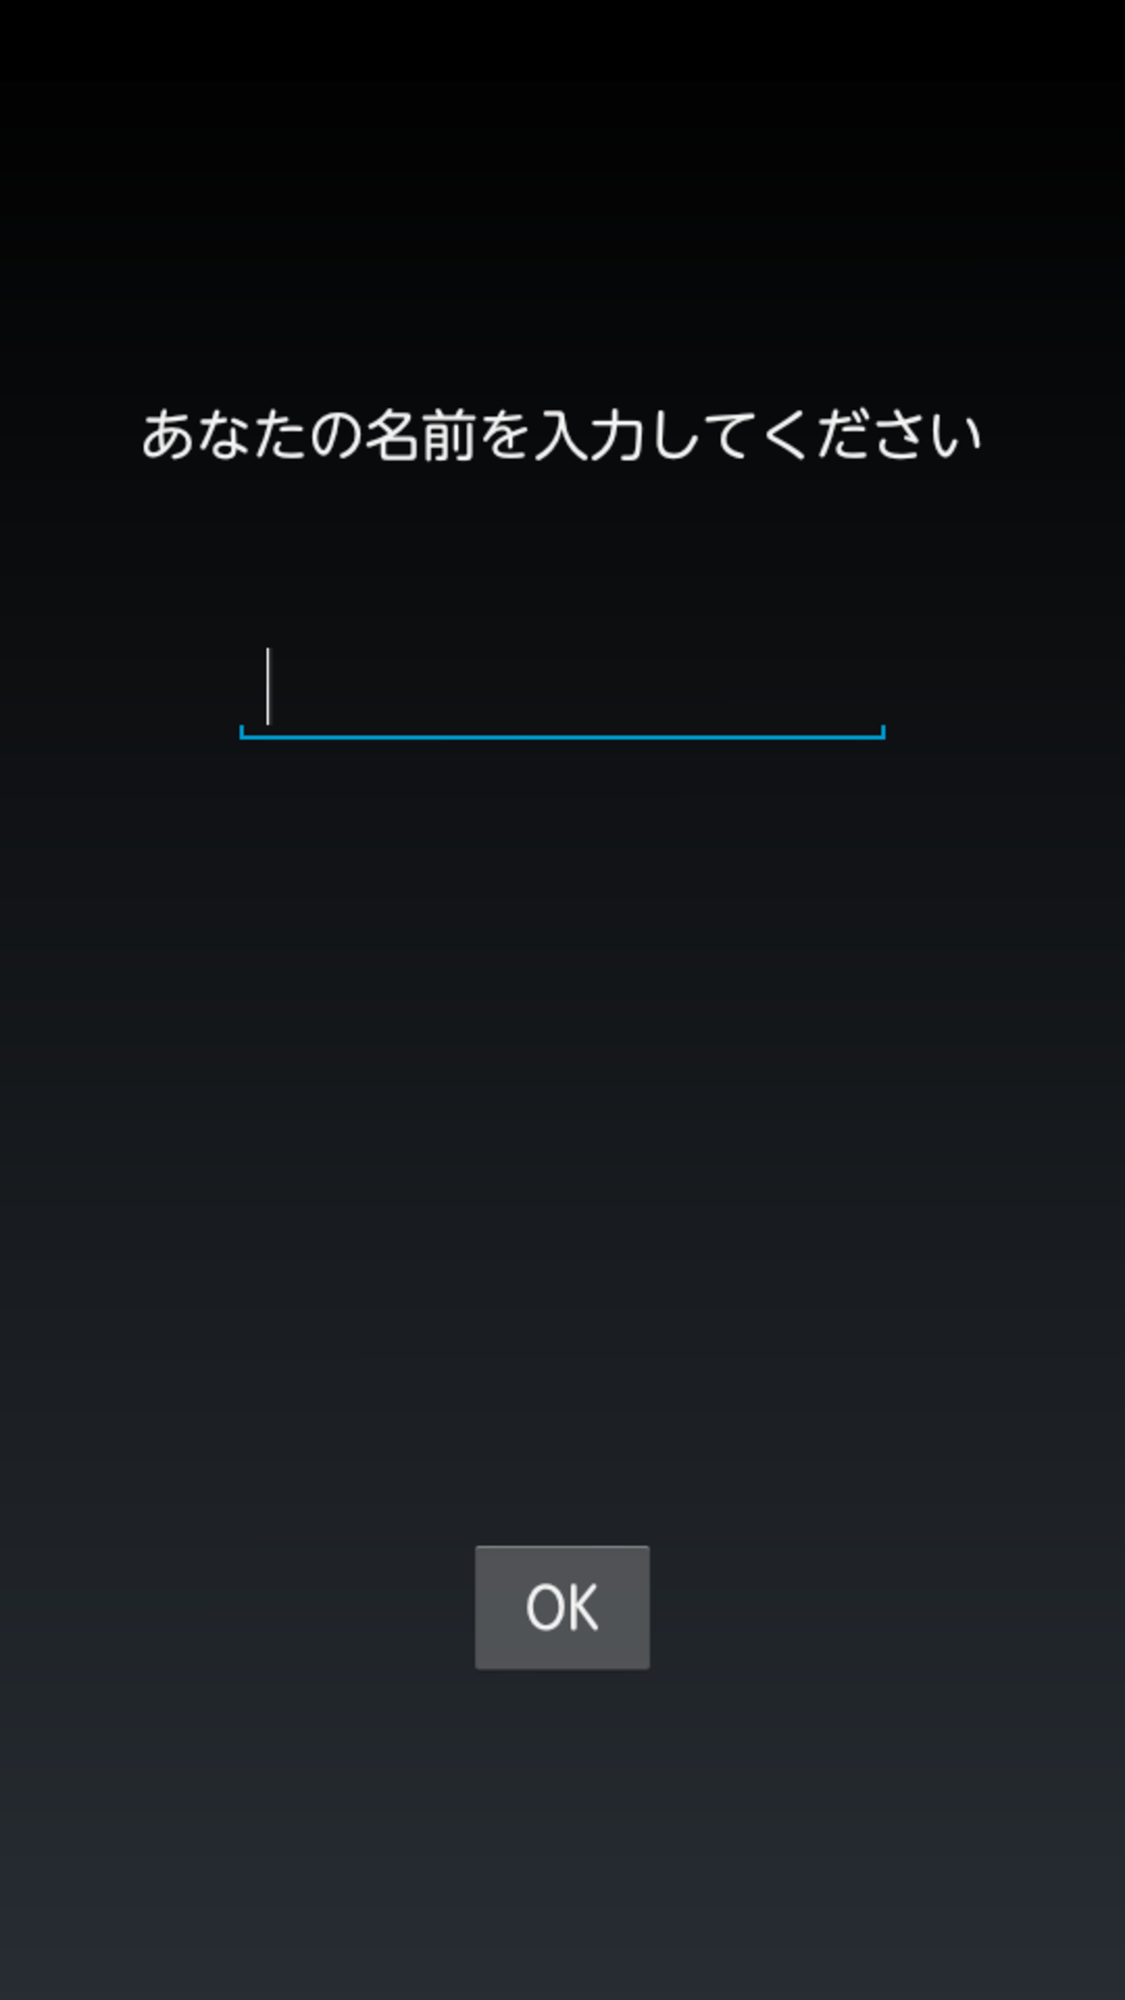
\includegraphics[width=5cm, bb=0 0 540 960]{NameInput.pdf}
                \end{center}
                \caption{ユーザ名入力画面}
                \label{authNameInput}
            \end{minipage}
            \begin{minipage}{0.33\hsize}
                \begin{center}
                    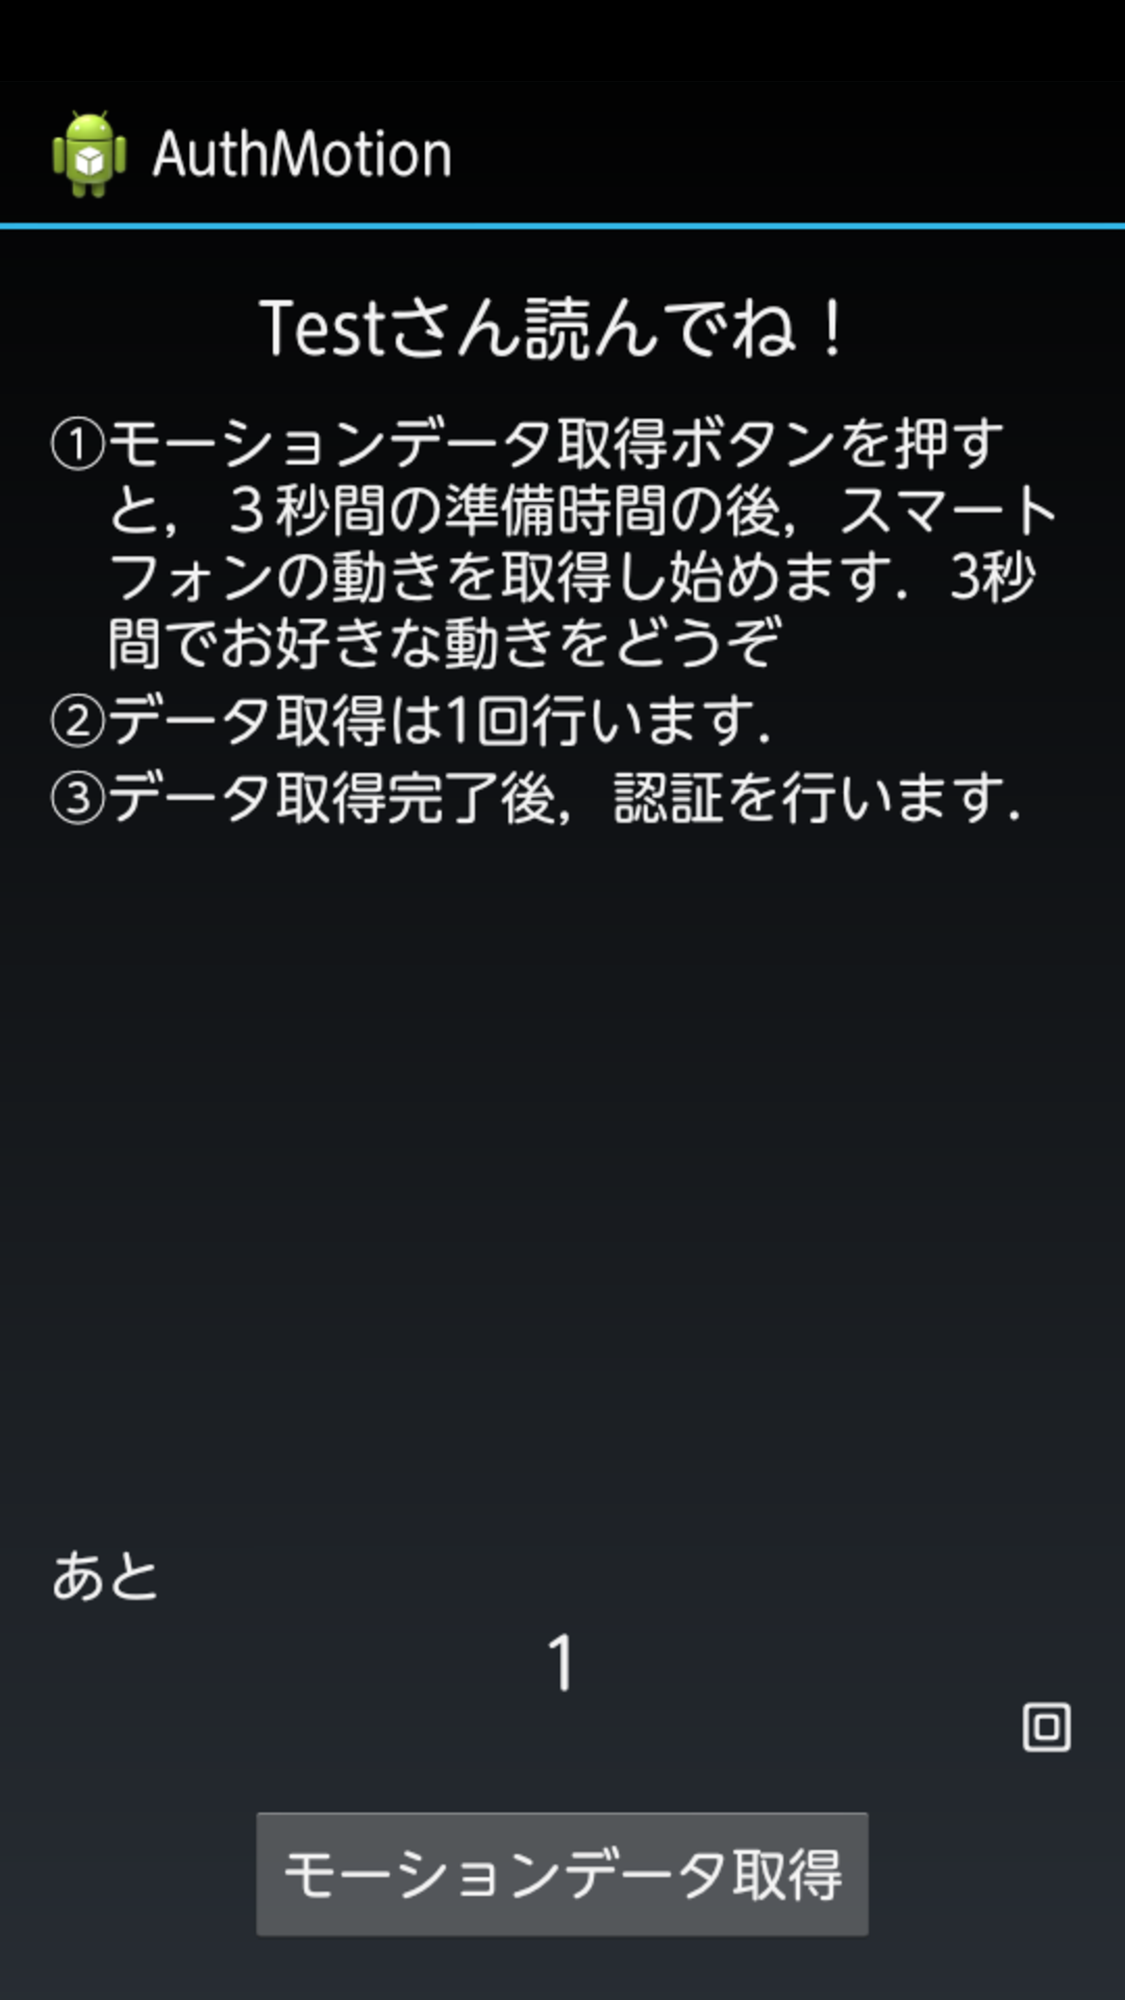
\includegraphics[width=5cm, bb=0 0 540 960]{Auth.pdf}
                \end{center}
                \caption{認証試験画面}
                \label{auth}
            \end{minipage}
            \begin{minipage}{0.33\hsize}
                \begin{center}
                    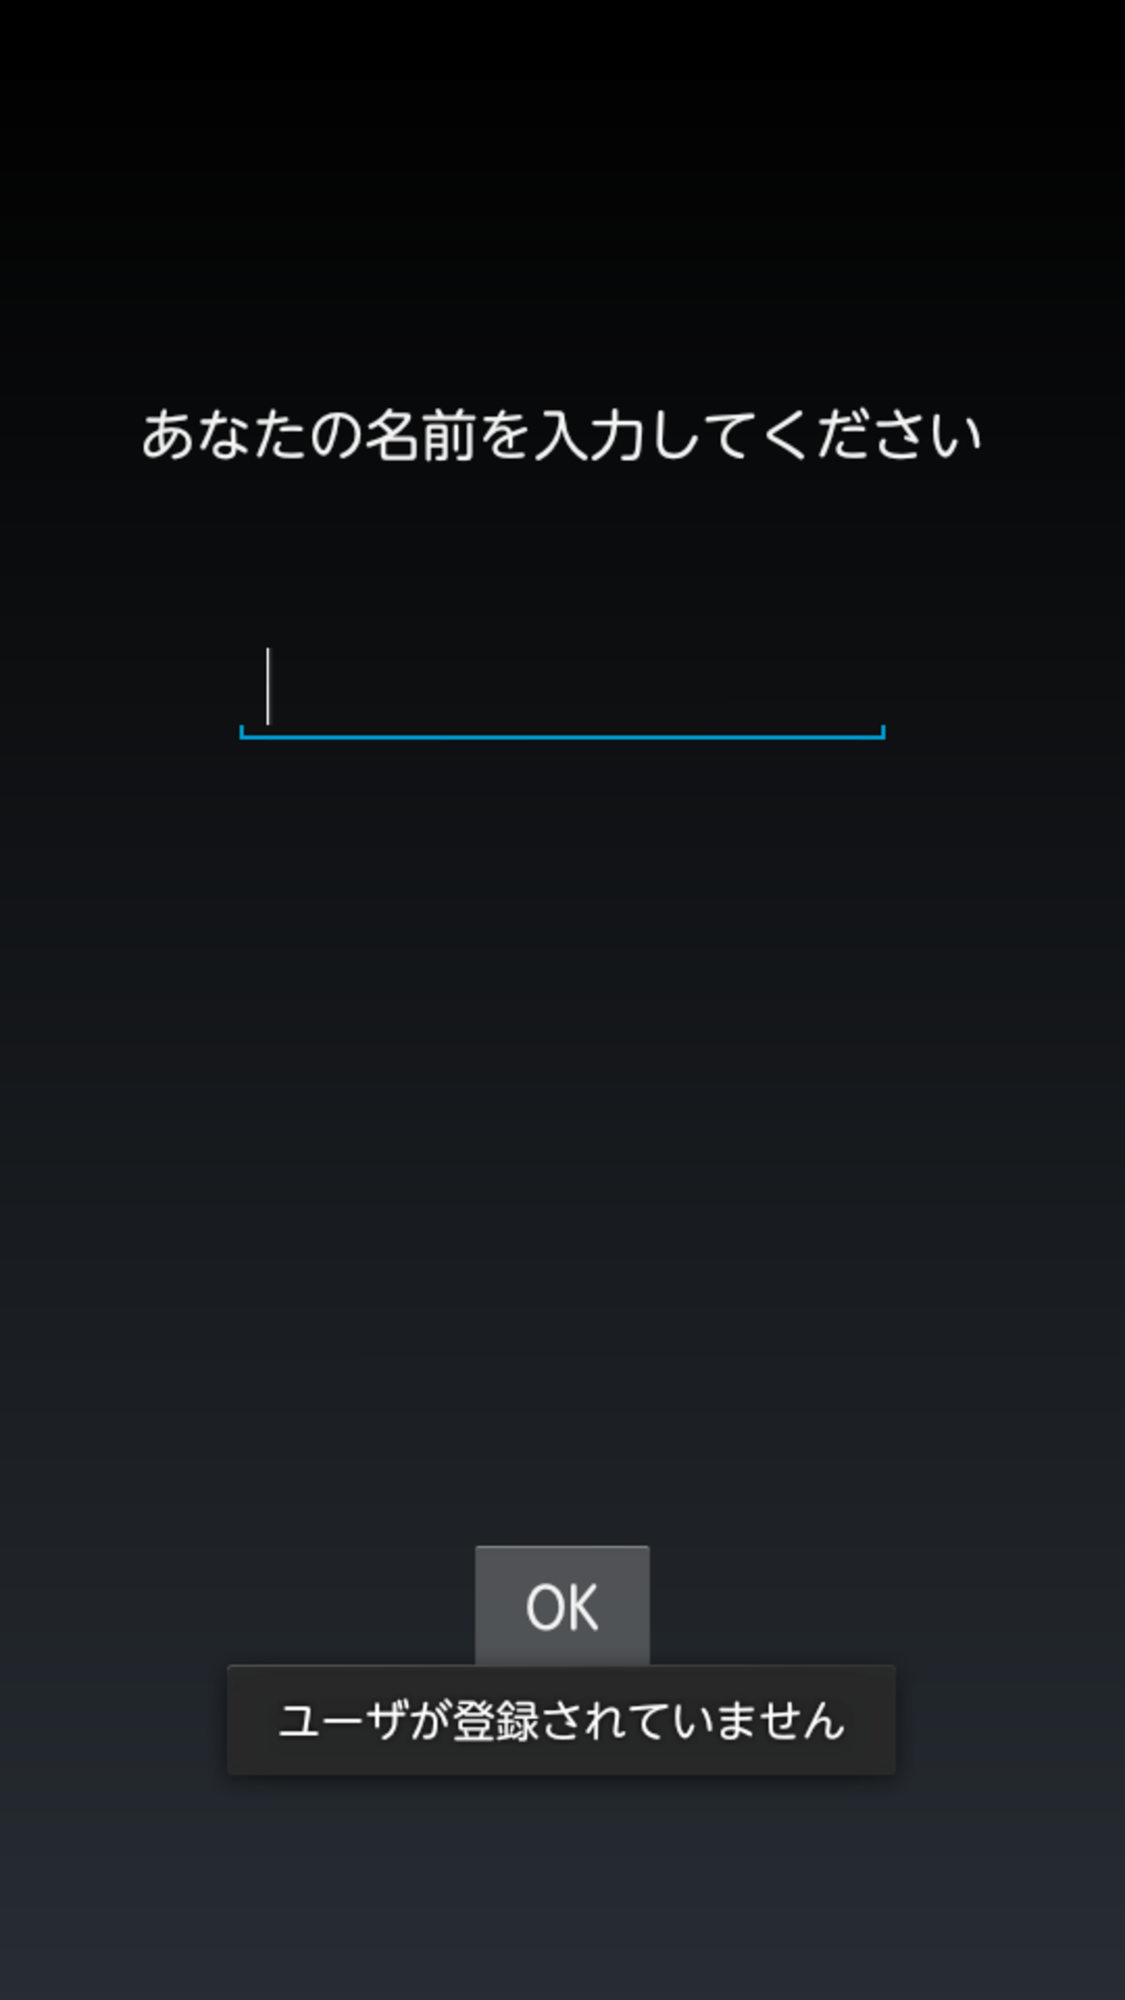
\includegraphics[width=5cm, bb=0 0 540 960]{AuthNameInputError.pdf}
                \end{center}
                \caption{エラー通知}
                \label{authNameInputError}
            \end{minipage}
        \end{figure}

        \newpage
        \lstinputlisting[caption=ユーザ確認, label=authCheckInputNameSource, style=MyJava]
        {Code\slash authCheckInputName}

        認証試験モードでは新規登録モードと異なり,1回分のモーションデータ取得を行う.
        モーションデータの取得後,新規登録モードにおいて登録された増幅量を元に取得したデータに対して増幅処理を行う.
        そして,フーリエ変換を用いたローパスフィルタ処理を行い,新規登録モードにおいて登録されたデータとの相関係数を算出し個人認証を行う.
        個人認証に成功すれば,図\ref{authSuccess}のような認証成功ダイアログを表示する.
        このダイアログのOKボタンを押すことで,起動画面へと移動する.
        個人認証に失敗すれば,図\ref{authFail}のような認証失敗ダイアログを表示する.
        このダイアログのOKボタンを押すことでプログラム内部のモーションデータ取得カウンタが初期化され,再度個人認証を行えるようにする.

        \begin{figure}[tbp]
            \begin{minipage}{0.5\hsize}
                \begin{center}
                    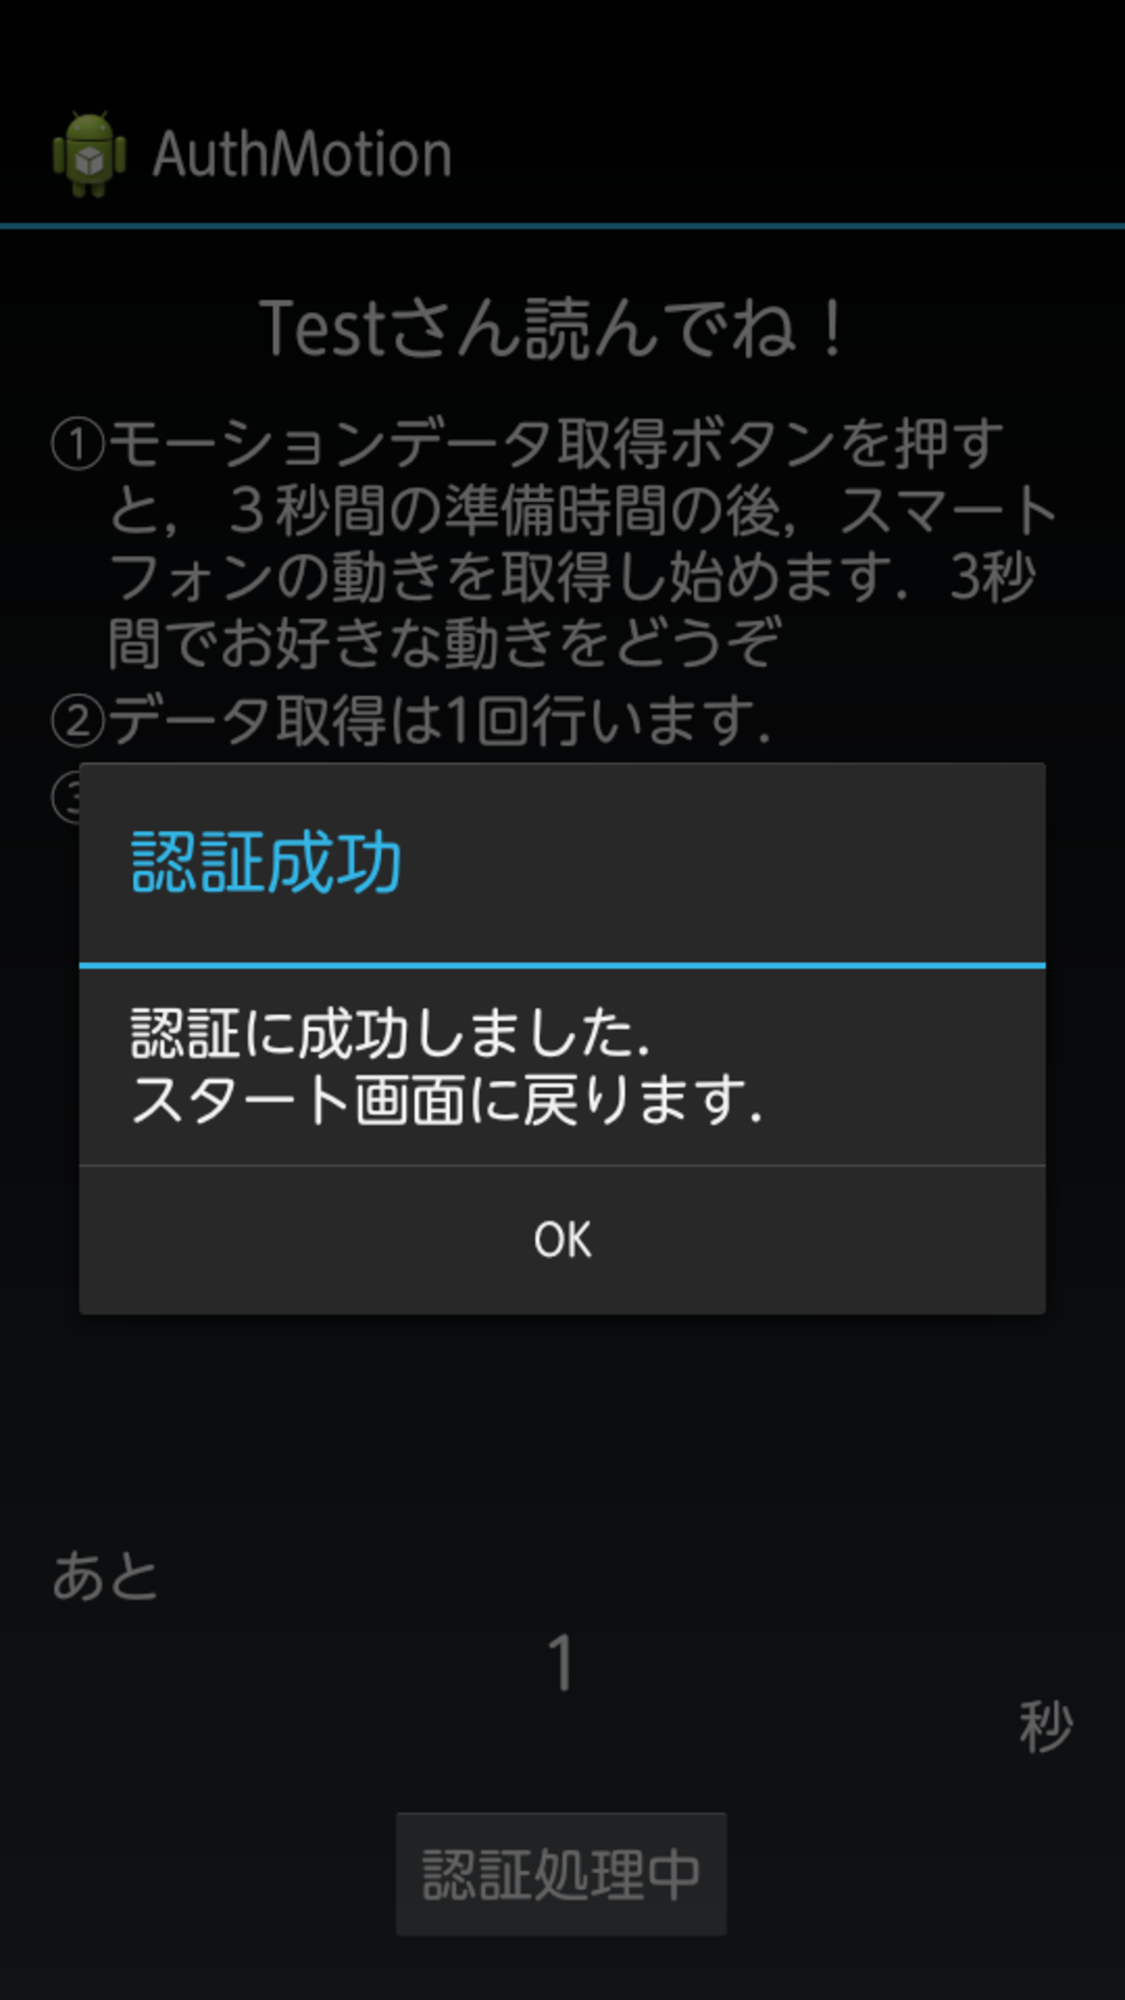
\includegraphics[width=5cm, bb=0 0 540 960]{AuthSuccess.pdf}
                \end{center}
                \caption{認証成功ダイアログ}
                \label{authSuccess}
            \end{minipage}
            \begin{minipage}{0.5\hsize}
                \begin{center}
                    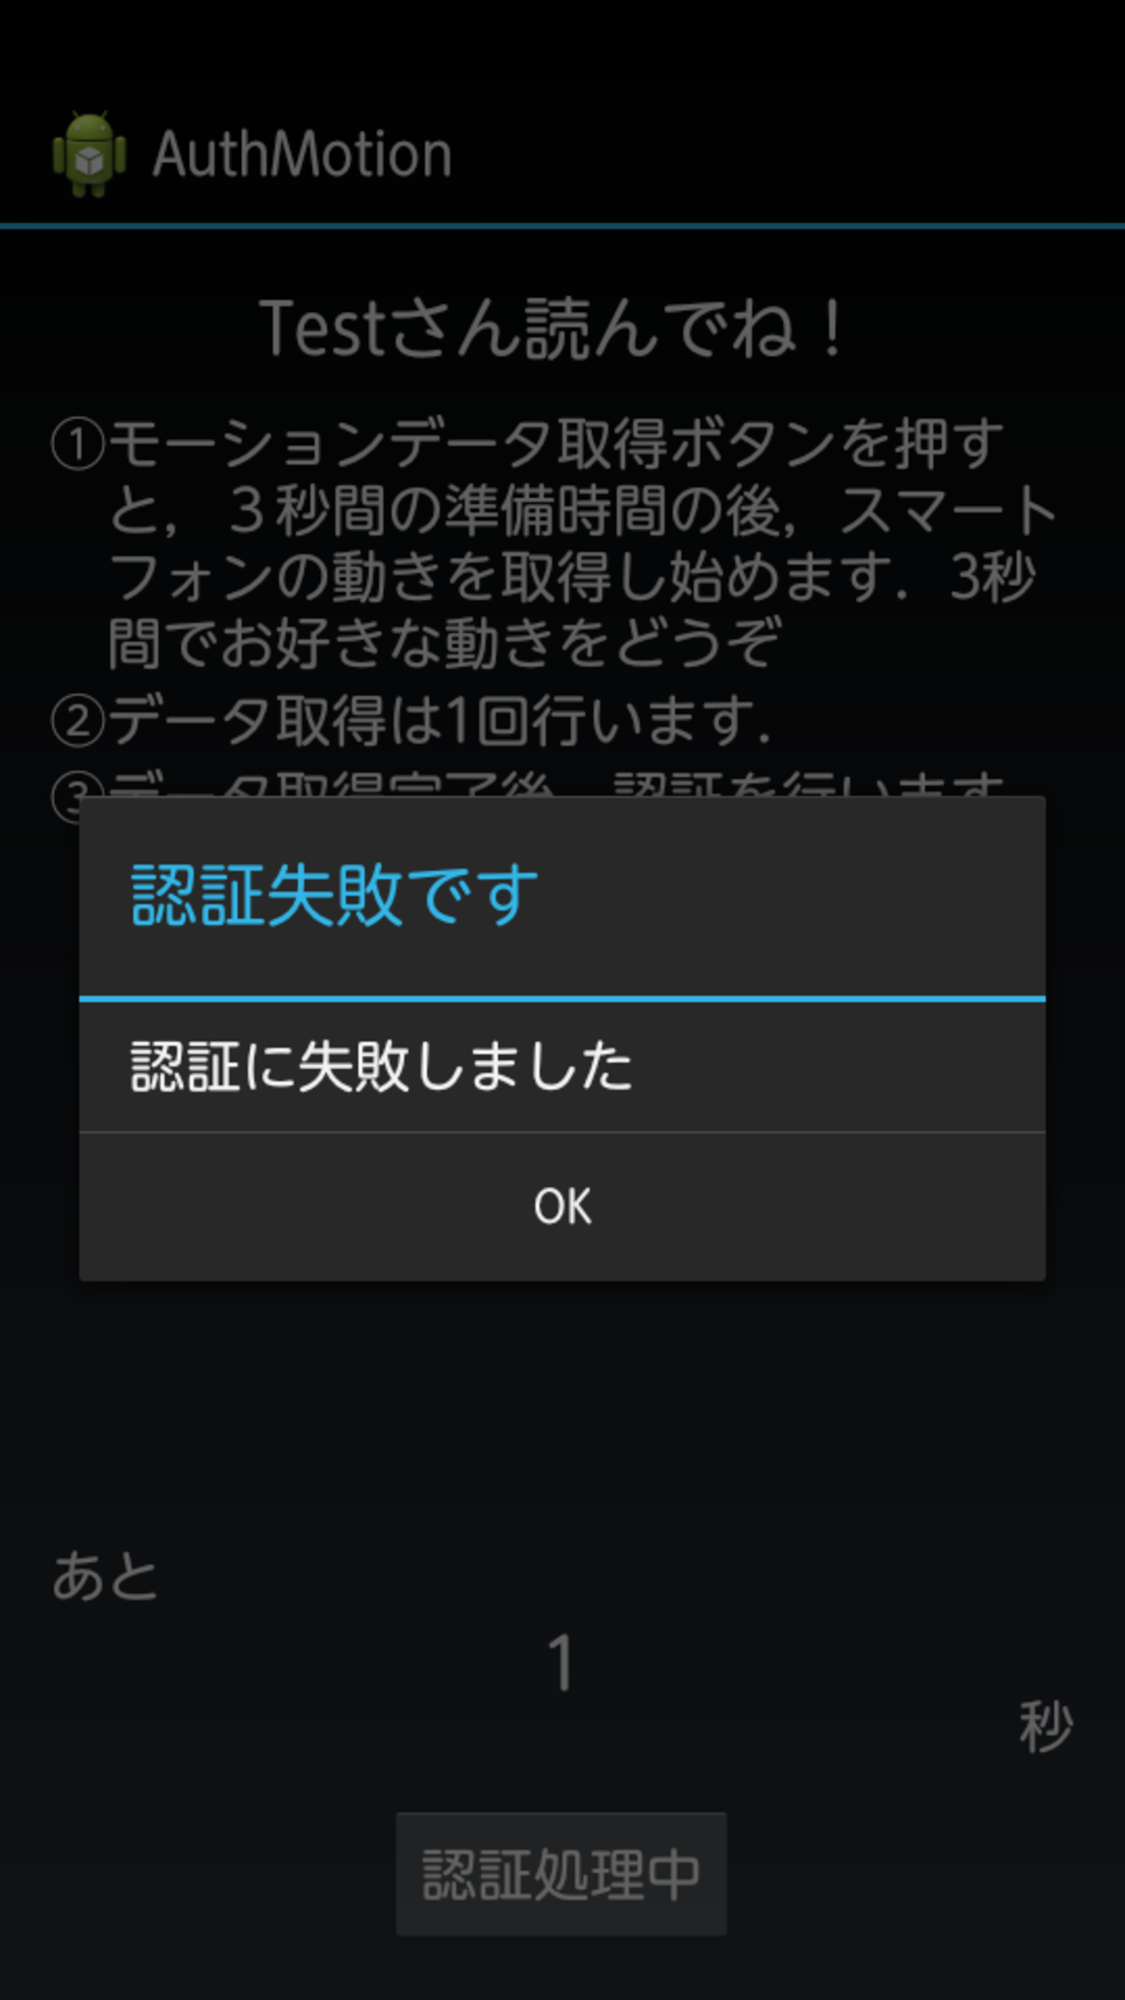
\includegraphics[width=5cm, bb=0 0 540 960]{AuthFail.pdf}
                \end{center}
                \caption{認証失敗ダイアログ}
                \label{authFail}
            \end{minipage}
        \end{figure}

% ^^^^^^^^^^^^^^^^^^^^^^^^^^^^^^^^^^^^^^^^^^^^^^^^^^^^^^^^^^
%                    データ閲覧モード
% vvvvvvvvvvvvvvvvvvvvvvvvvvvvvvvvvvvvvvvvvvvvvvvvvvvvvvvvvv
        \subsection{データ閲覧モード}
        % 表現を改良する必要があるかもしれない
        データ閲覧モードでは,新規登録モードにおいて登録されたユーザ名とそれぞれのユーザが登録したモーションデータを閲覧することが出来る.
        このモードを選択すると,まず図\ref{userList}のようなユーザ名の一覧が表示される.
        ここでデータを閲覧したいユーザ名を選択することで,図\ref{dataList}のようにモーションを調べることが出来る.

        \begin{figure}[tbp]
            \begin{minipage}{0.5\hsize}
                \begin{center}
                    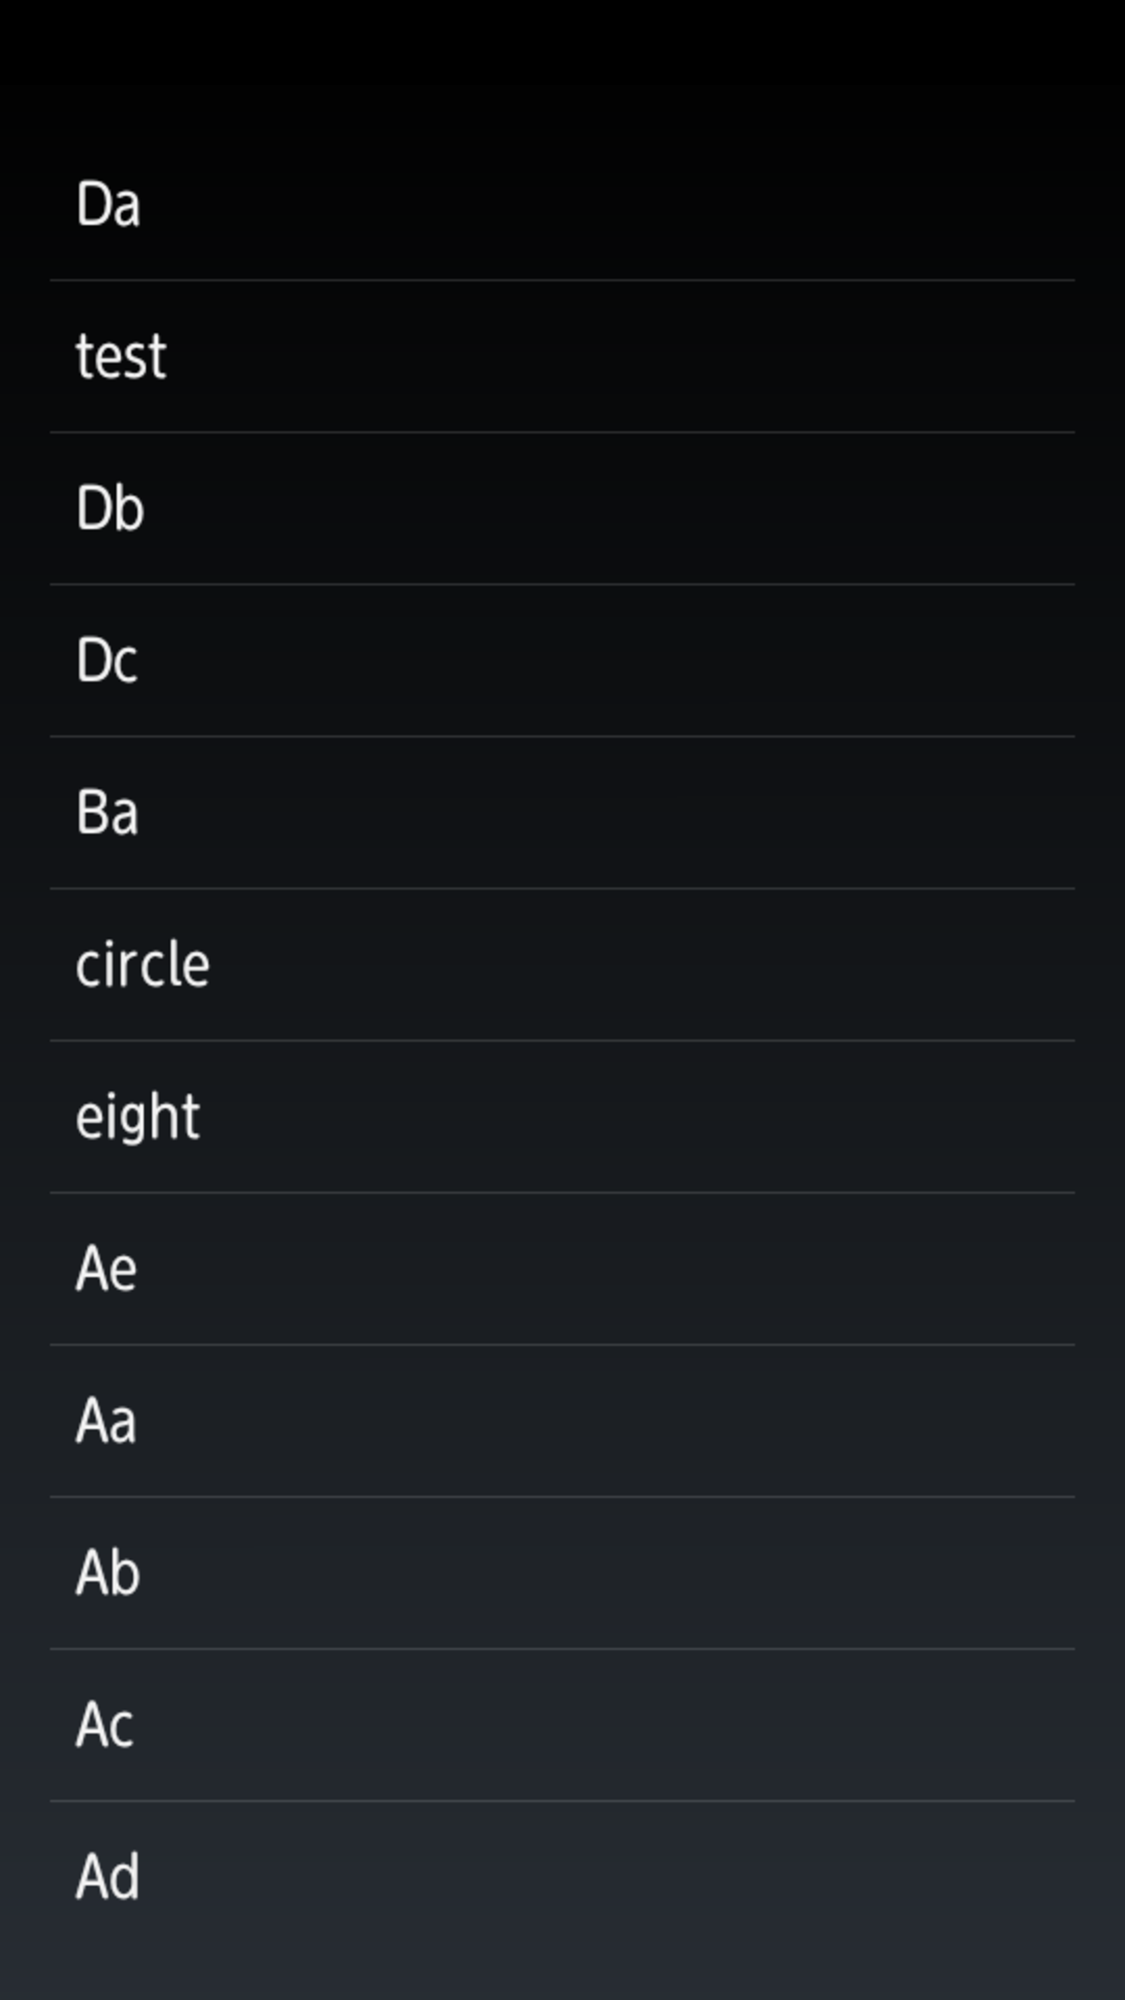
\includegraphics[width=5cm, bb=0 0 540 960]{UserList.pdf}
                \end{center}
                \caption{ユーザ名一覧画面}
                \label{userList}
            \end{minipage}
            \begin{minipage}{0.5\hsize}
                \begin{center}
                    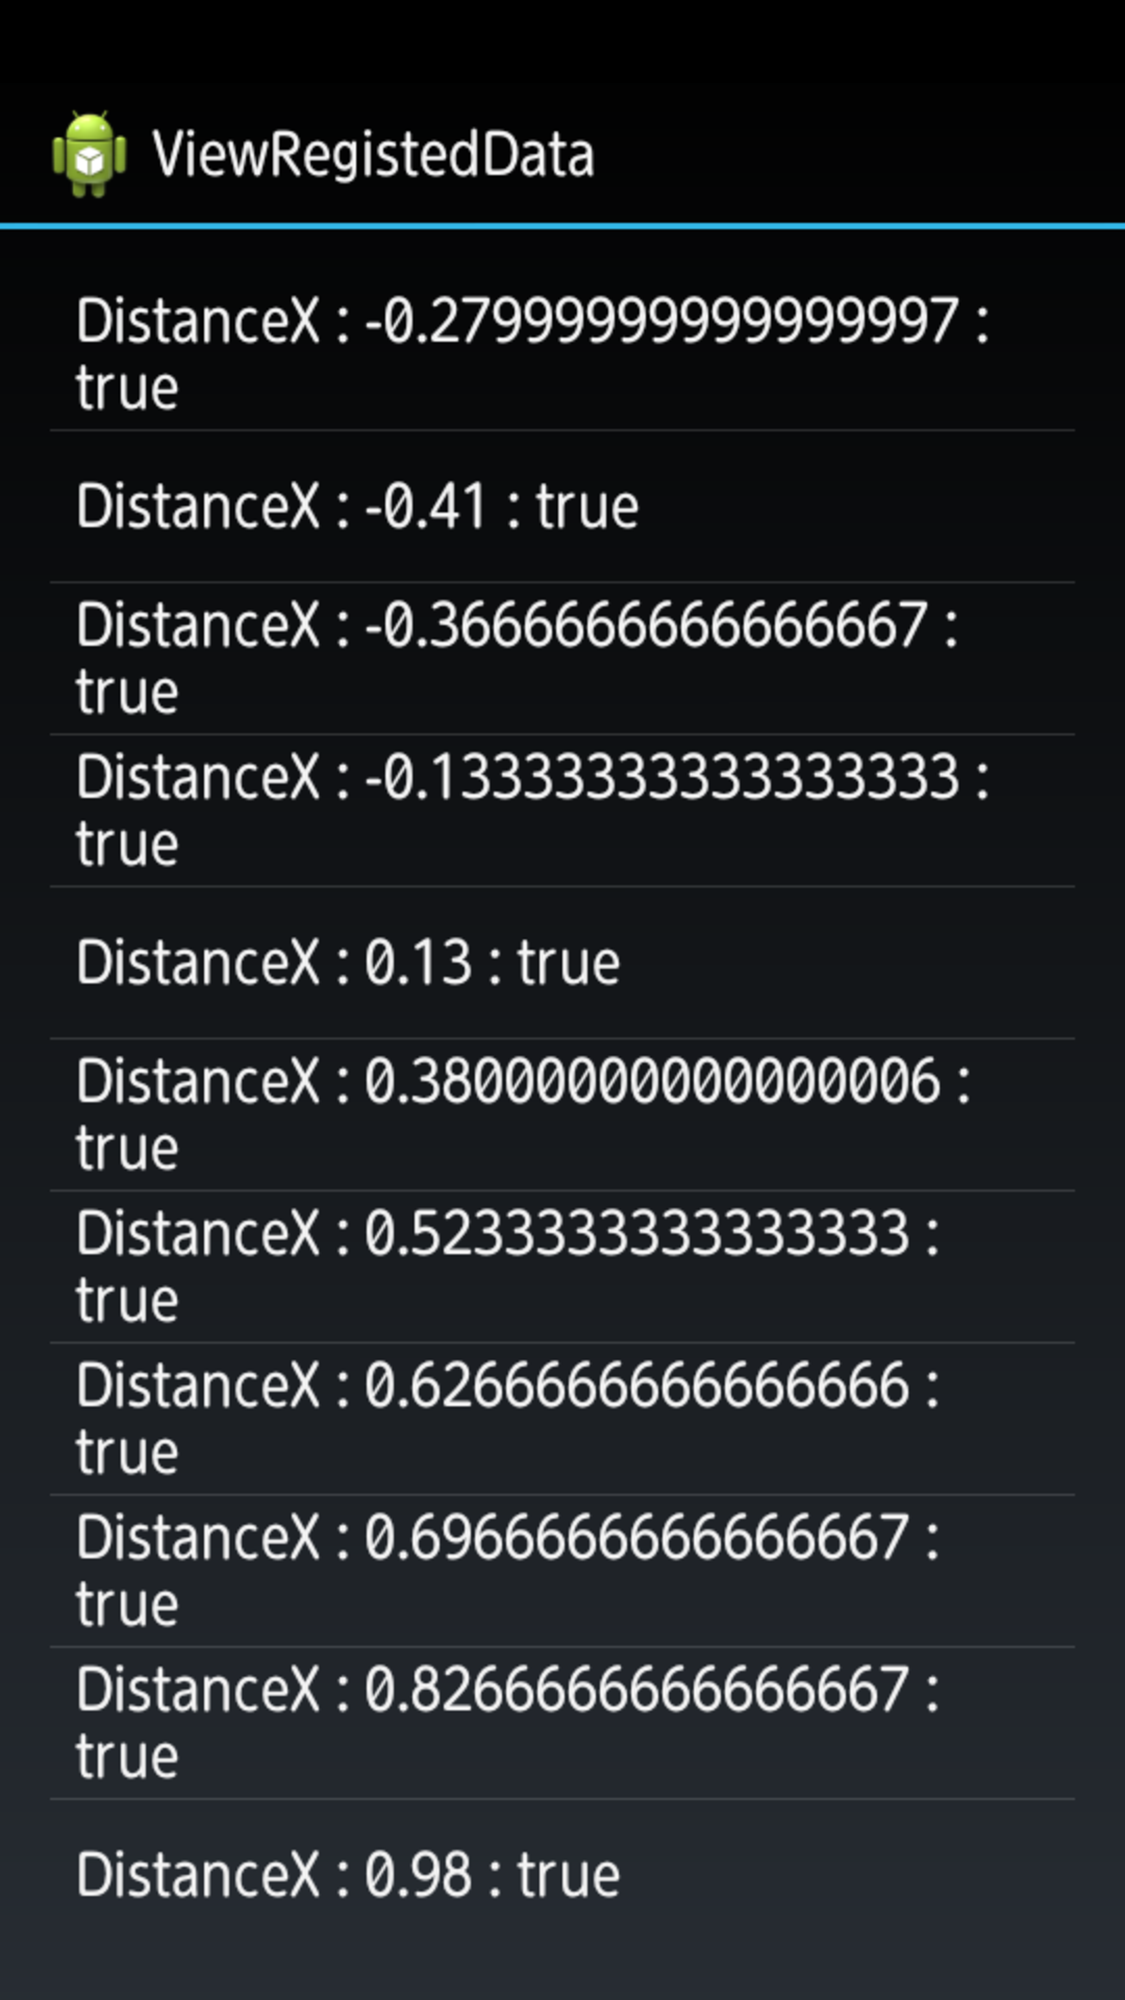
\includegraphics[width=5cm, bb=0 0 540 960]{DataList.pdf}
                \end{center}
                \caption{モーションデータ一覧画面}
                \label{dataList}
            \end{minipage}
        \end{figure}

% ^^^^^^^^^^^^^^^^^^^^^^^^^^^^^^^^^^^^^^^^^^^^^^^^^^^^^^^^^^
% ^^^^^^^^^^^^^^^^^^^^^^^^^^^^^^^^^^^^^^^^^^^^^^^^^^^^^^^^^^
%                    先行研究からの改善点
% vvvvvvvvvvvvvvvvvvvvvvvvvvvvvvvvvvvvvvvvvvvvvvvvvvvvvvvvvv
% vvvvvvvvvvvvvvvvvvvvvvvvvvvvvvvvvvvvvvvvvvvvvvvvvvvvvvvvvv
    \section{先行研究からの改善点}
    先行研究において指摘されていた,手首のスナップを用いるような比較的動きの小さなモーションにおいて,認証率が低く出てしまうという課題を解決するために導入した機能をここに挙げる.

% ^^^^^^^^^^^^^^^^^^^^^^^^^^^^^^^^^^^^^^^^^^^^^^^^^^^^^^^^^^
%                モーションデータの増幅機能
% vvvvvvvvvvvvvvvvvvvvvvvvvvvvvvvvvvvvvvvvvvvvvvvvvvvvvvvvvv
        \subsection{モーションデータの増幅機能}
        手首を中心とするような動きの小さいモーションにおける個人認証成功率を向上させるために,モーションデータの増幅機能を実装した.
        これにより,比較的動きの小さなモーションであってもデータを増幅して用いることができ,比較的動きの大きなモーションと比べて遜色なく用いることが出来るようになった.
        この処理をソースコード\ref{amplifierSource}に示す.

        \lstinputlisting[caption=モーションデータ増幅機能, label=amplifierSource, style=MyJava]
        {Code\slash amplifier}

        この増幅機能は,事前にデータの最大値と最小値の差を取り,得られた値があらかじめ設定された閾値を下回った場合にのみ機能するようにしている.
        この処理をソースコード\ref{dataRangeCheckSource}に示す.

        \lstinputlisting[caption=データレンジチェック, label=dataRangeCheckSource, style=MyJava]
        {Code\slash dataRangeCheck}

        データをどれだけ増幅させるかを決める値やデータの最大値と最小値の差がどれだけあれば増幅を行うかを決める閾値に関しては,新規登録モードにおいてメニューキーを押すことで表示される図\ref{regMenu}のようなメニュー内の増幅器設定を選択することで表示される,図\ref{amplifierSettings}のような設定ダイアログより変更することが出来る.

    \begin{figure}[!bhtp]
        \begin{minipage}{0.5\hsize}
            \begin{center}
                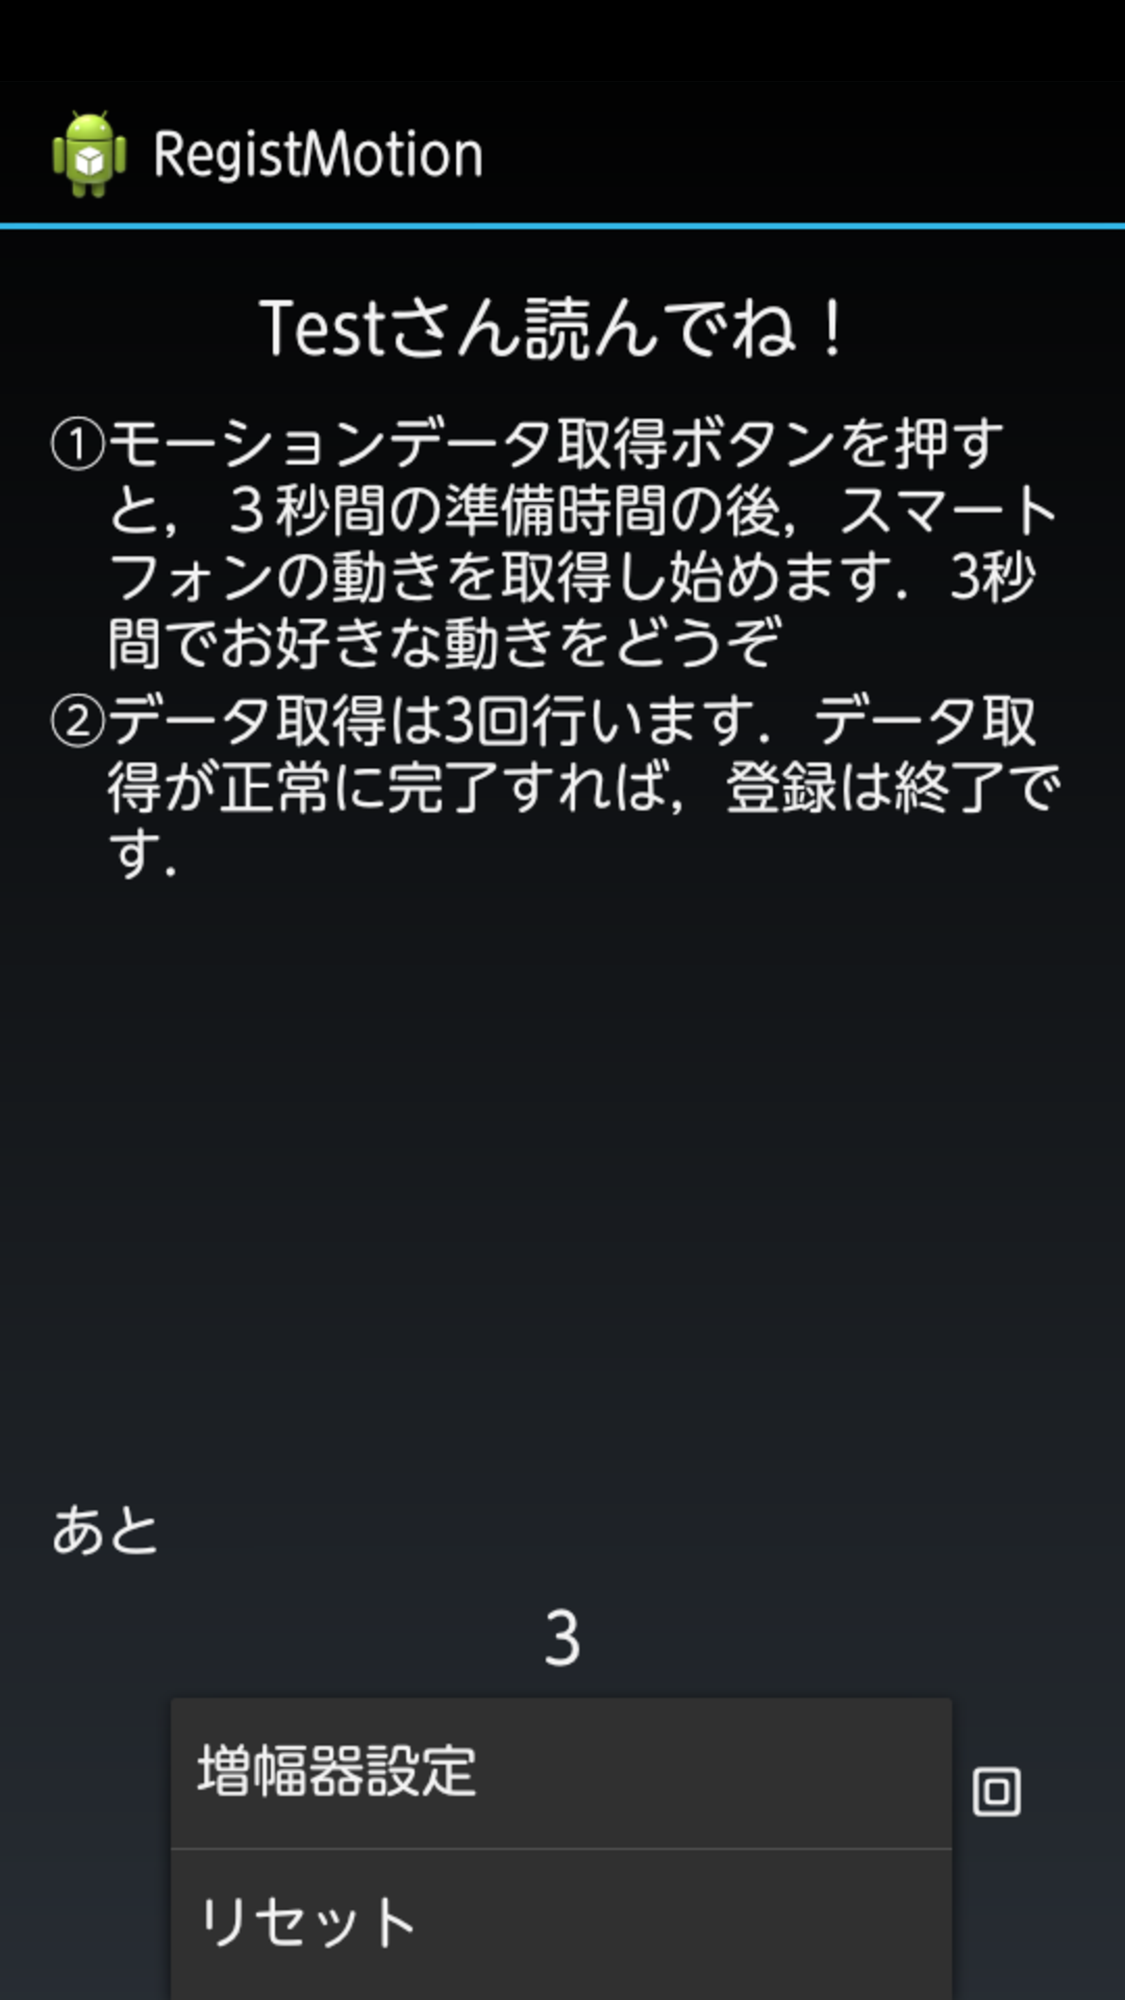
\includegraphics[width=5cm, bb=0 0 540 960]{RegMenu.pdf}
            \end{center}
            \caption{新規登録モードメニュー画面}
            \label{regMenu}
        \end{minipage}
        \begin{minipage}{0.5\hsize}
            \begin{center}
                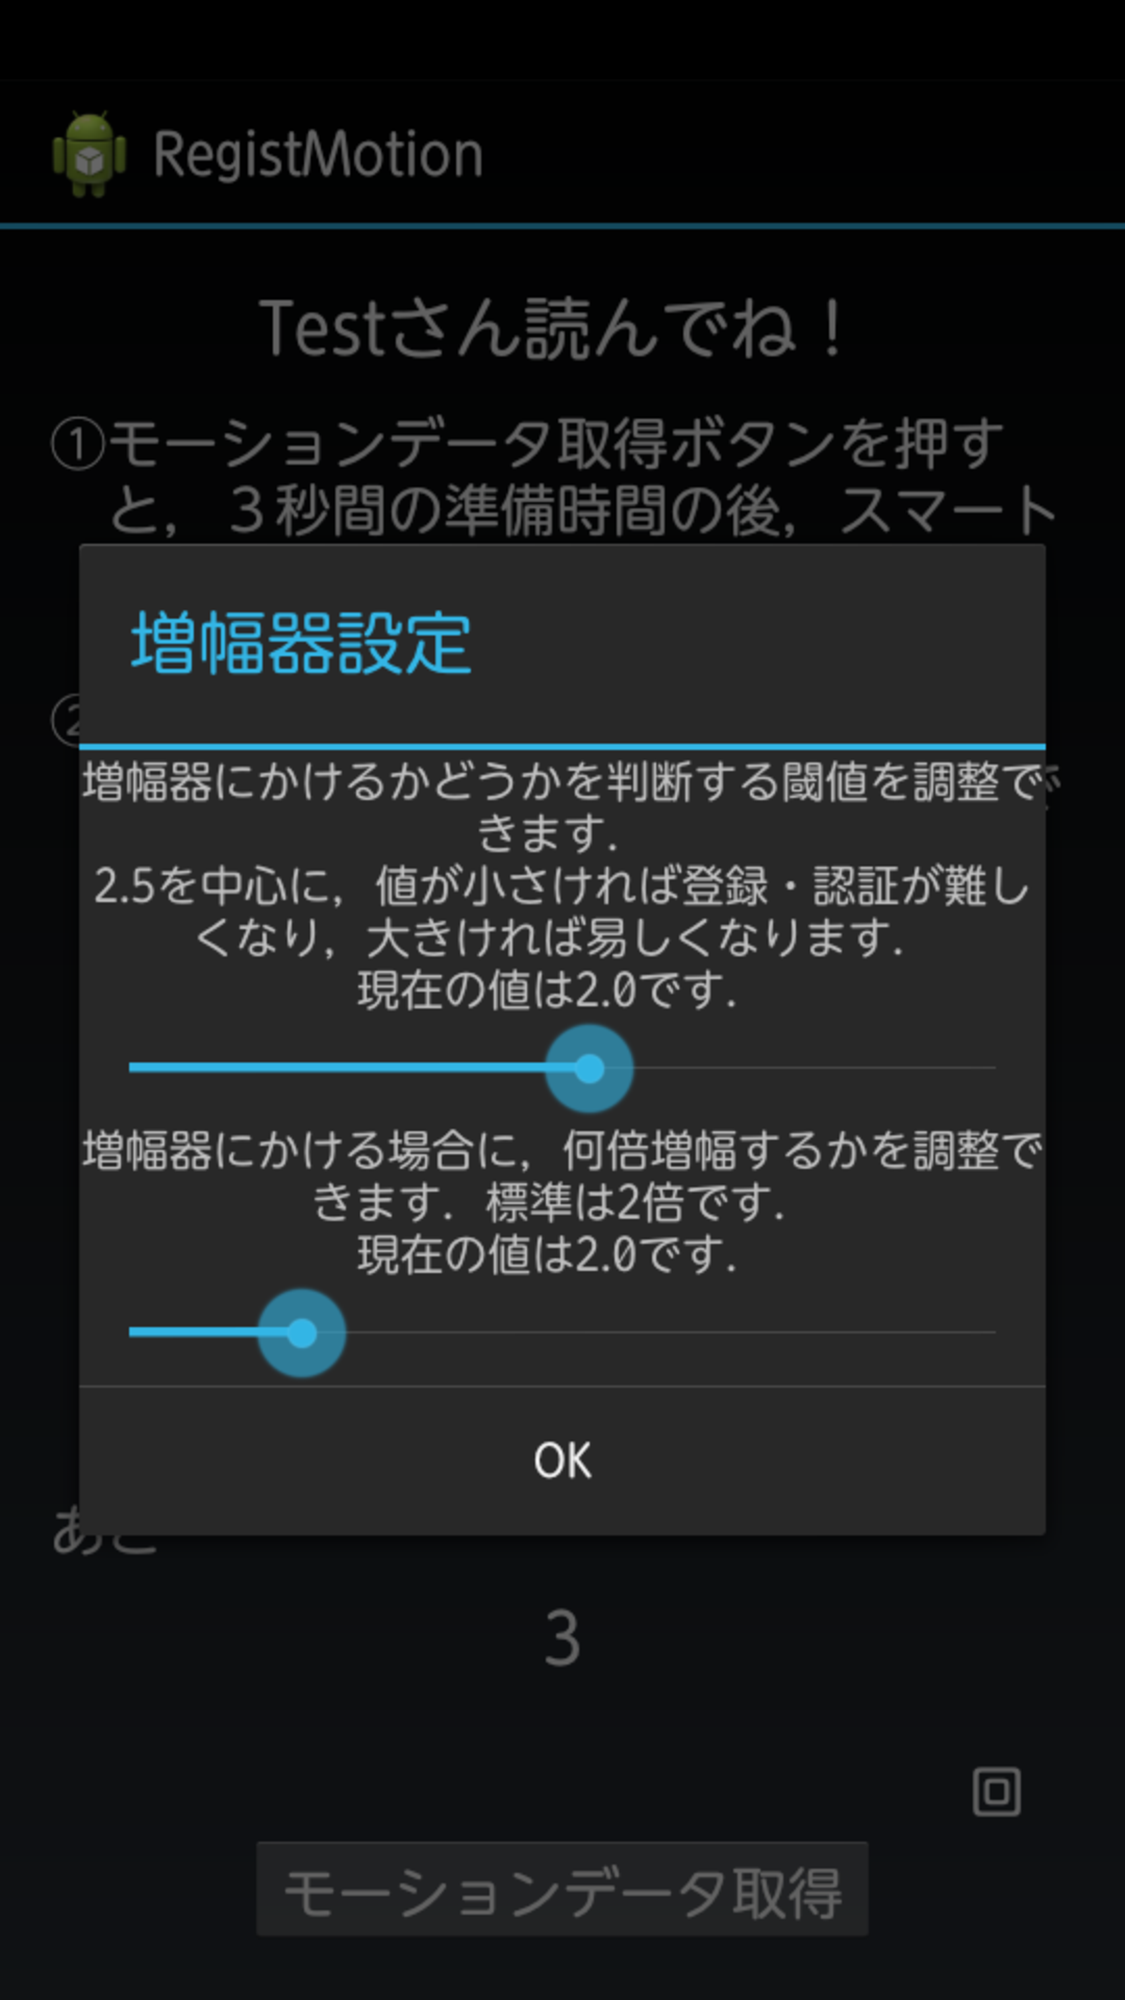
\includegraphics[width=5cm, bb=0 0 540 960]{AmplifierSettings.pdf}
            \end{center}
            \caption{増幅器設定ダイアログ}
            \label{amplifierSettings}
        \end{minipage}
    \end{figure}

        増幅器にかける前のデータをグラフ化したものを図\ref{beforeAmpDataGraph}に,かけた後のデータをグラフ化したものを図\ref{afterAmpDataGraph}に示す.
        % Data : BeforeAMP and AfterAMP

        \begin{figure}[btp]
            \begin{minipage}{0.5\hsize}
                \begin{center}
                    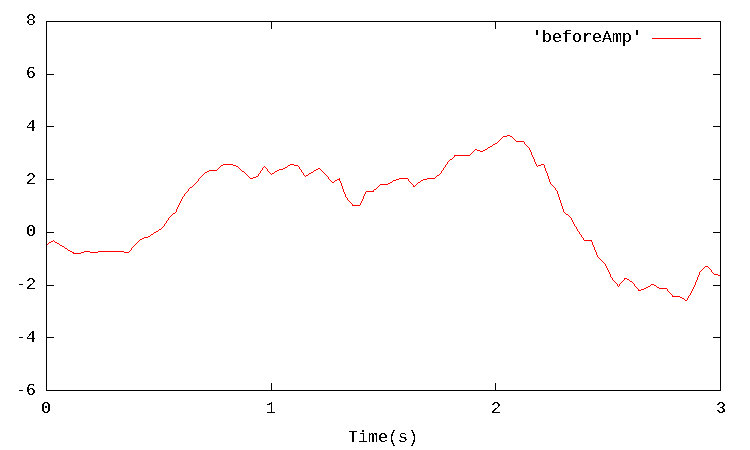
\includegraphics[width=8cm, bb=0 0 360 216]{beforeAmpGraph.pdf}
                \end{center}
                \caption{増幅前のデータ}
                \label{beforeAmpDataGraph}
            \end{minipage}
            \begin{minipage}{0.5\hsize}
                \begin{center}
                    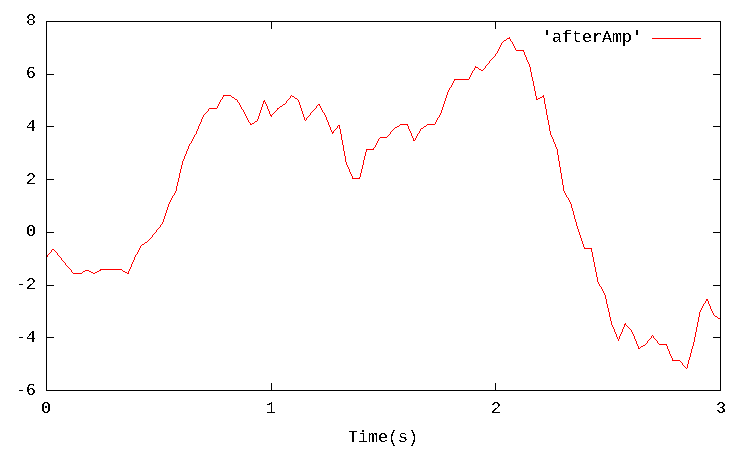
\includegraphics[width=8cm, bb=0 0 360 216]{afterAmpGraph.pdf}
                \end{center}
                \caption{増幅後のデータ}
                \label{afterAmpDataGraph}
            \end{minipage}
        \end{figure}

% ^^^^^^^^^^^^^^^^^^^^^^^^^^^^^^^^^^^^^^^^^^^^^^^^^^^^^^^^^^
%           フーリエ変換を用いたローパスフィルタ
% vvvvvvvvvvvvvvvvvvvvvvvvvvvvvvvvvvvvvvvvvvvvvvvvvvvvvvvvvv
        \subsection{フーリエ変換を用いたローパスフィルタ}
        モーションデータを取得している際の細かな手の震えなどによるデータに対する影響を取り除き,モーションデータとしての純度を高めるために,フーリエ変換を用いたローパスフィルタ処理を行っている.

        フーリエ変換を用いて時間軸で表されるモーションデータを周波数領域に変換することで,モーション中の細かな手の震えなどのデータが高周波成分として現れる.
        そしてこの高周波成分を取り除いた上で元の時間軸のデータに戻すローパスフィルタ処理を行うことで,細かな手の震えなどによるデータに対する影響を取り除いている.
        フーリエ変換を実装する際には,CERNのColt Project\cite{coltproj}で開発されたJavaによる科学技術計算用ライブラリであるColt\cite{colt}をマルチスレッド化したParallel Colt\cite{parallelcolt}に含まれている,JTransforms\cite{jtransforms}を用いて実装している.
        この処理をソースコード\ref{lowpassSource}に示す.

        % 付録に回す
        \lstinputlisting[caption=ローパスフィルタ処理, label=lowpassSource, style=MyJava]
        {Code\slash lowpass}

        ローパスフィルタにかける前のデータをグラフ化したものを図\ref{beforeLowpassDataGraph}に,かけた後のデータをグラフ化したものを図\ref{afterLowpassDataGraph}に示す.

        \begin{figure}[!bhtp]
            \begin{minipage}{0.5\hsize}
                \begin{center}
                    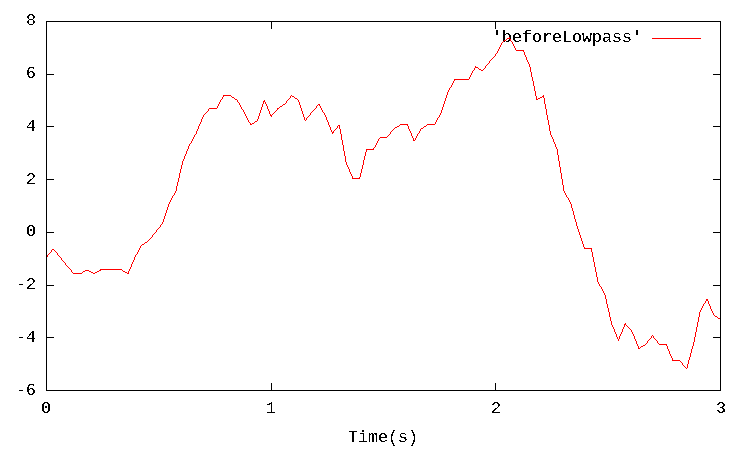
\includegraphics[width=8cm, bb=0 0 360 216]{beforeLowpassGraph.pdf}
                \end{center}
                \caption{ローパスフィルタ前のデータ}
                \label{beforeLowpassDataGraph}
            \end{minipage}
            \begin{minipage}{0.5\hsize}
                \begin{center}
                    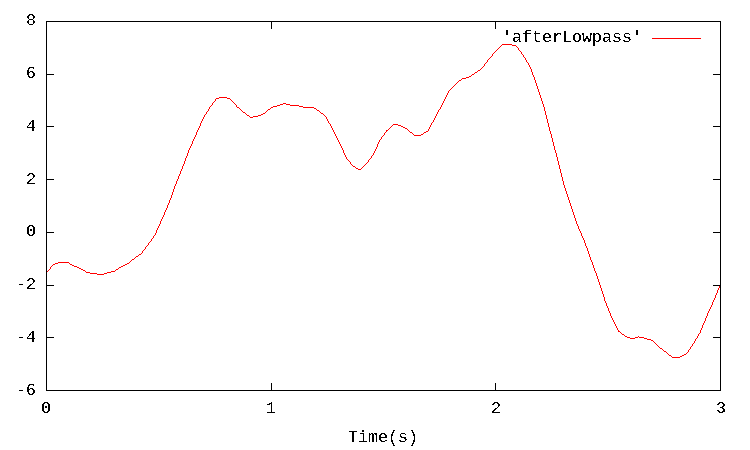
\includegraphics[width=8cm, bb=0 0 360 216]{afterLowpassGraph.pdf}
                \end{center}
                \caption{ローパスフィルタ後のデータ}
                \label{afterLowpassDataGraph}
            \end{minipage}
        \end{figure}

% ^^^^^^^^^^^^^^^^^^^^^^^^^^^^^^^^^^^^^^^^^^^^^^^^^^^^^^^^^^
%          モーション取得時のズレを修正する機能
% vvvvvvvvvvvvvvvvvvvvvvvvvvvvvvvvvvvvvvvvvvvvvvvvvvvvvvvvvv
        \subsection{モーション取得時のズレを修正する機能}
        新規登録モードにおいてモーションを登録する際には3回分のモーションデータの入力が必要になるが,この回数ごとにモーションの時間的なズレが生じた場合はデータ登録や認証時に影響を与えてしまう可能性があるため,このズレを修正する処理を3回分のデータ取得後に行うようにしている.

        3回分のデータ取得後,まずはこのデータ間の相関係数を算出し,回数ごとに全く別のモーションが入力されていないかの確認を行う.
        そしてある程度以上の相関が見られるが,それでも相関係数が低く出てしまった場合に,ズレ修正後の相関係数を確認しつつ,データの最大値に合わせるパターン,データの最小値に合わせるパターン,データの中央値に合わせるパターンの最大三つの方法で相関係数の向上を試みる.
        この部分の処理を付録のソースコード\ref{checkDeviationSource}に示す.

        相関係数を算出した結果,ズレ修正が必要であると判断された場合,付録のソースコード\ref{correctDeviationSource}に示したズレ修正アルゴリズムを用いて修正を行う.

        ズレ修正を行う前のデータをグラフ化したものを図\ref{beforeDeviationDataGraph}に,修正を行った後のデータをグラフ化したものを図\ref{afterDeviationDataGraph}に示す.

        % 修正前と修正後の比較グラフ
        \begin{figure}[btp]
            \begin{minipage}{0.5\hsize}
                \begin{center}
                    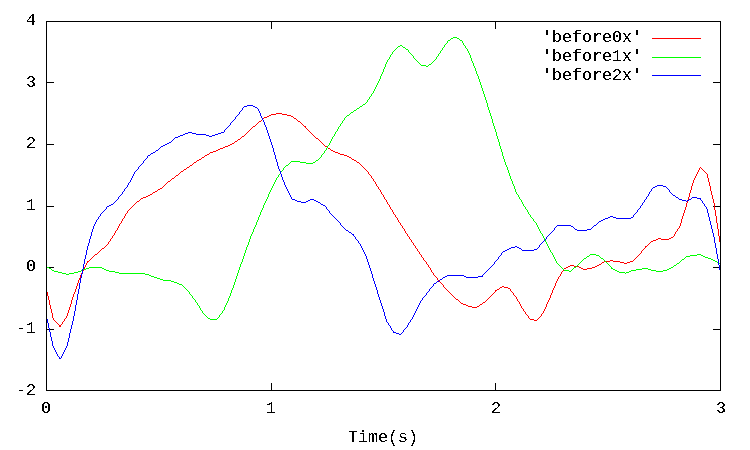
\includegraphics[width=8cm, bb=0 0 360 216]{beforeDeviationGraph.pdf}
                \end{center}
                \caption{ズレ修正前のデータ}
                \label{beforeDeviationDataGraph}
            \end{minipage}
            \begin{minipage}{0.5\hsize}
                \begin{center}
                    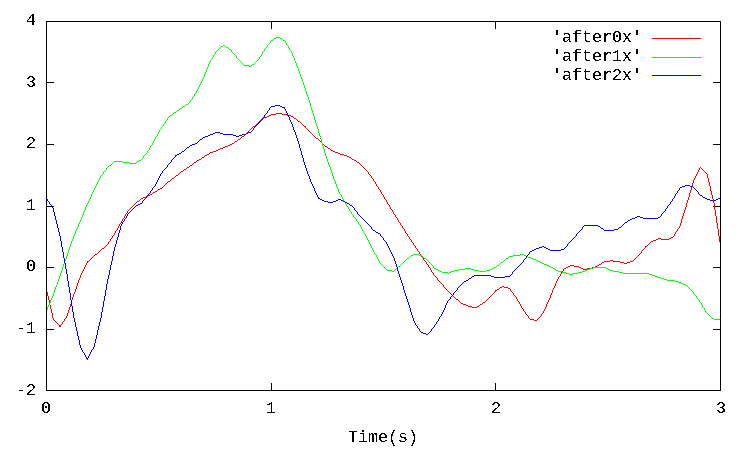
\includegraphics[width=8cm, bb=0 0 360 216]{afterDeviationGraph.pdf}
                \end{center}
                \caption{ズレ修正後のデータ}
                \label{afterDeviationDataGraph}
            \end{minipage}
        \end{figure}

        \subsection{モーション取得時のインターバル及びヴァイブレーション機能}
        新規登録モード及び認証試験モードにおいてモーション取得時の時間経過が把握しやすいように,1秒毎に端末をヴァイブレーションさせる機能を実装した.
        また,データ取得前のインターバルからデータ取得に移る際には通常より長めのヴァイブレーションにすることで,データ取得開始のタイミングを明確に意識できるようにした.

% ^^^^^^^^^^^^^^^^^^^^^^^^^^^^^^^^^^^^^^^^^^^^^^^^^^^^^^^^^^
% ^^^^^^^^^^^^^^^^^^^^^^^^^^^^^^^^^^^^^^^^^^^^^^^^^^^^^^^^^^
%                      実験と考察
% vvvvvvvvvvvvvvvvvvvvvvvvvvvvvvvvvvvvvvvvvvvvvvvvvvvvvvvvvv
% vvvvvvvvvvvvvvvvvvvvvvvvvvvvvvvvvvvvvvvvvvvvvvvvvvvvvvvvvv
\chapter{実験と考察}
    %\section{実験方法}
% ^^^^^^^^^^^^^^^^^^^^^^^^^^^^^^^^^^^^^^^^^^^^^^^^^^^^^^^^^^
%            新規登録及び個人認証の精度確認実験
% vvvvvvvvvvvvvvvvvvvvvvvvvvvvvvvvvvvvvvvvvvvvvvvvvvvvvvvvvv
    \section{新規登録及び個人認証の精度確認実験}
    \label{previousExp}
    手首のスナップを用いるような比較的小さなモーションにおける本システムの動作精度を確かめるために,新規登録および個人認証の成功率と成功時の平均試行回数を求める実験を行った.
    実験を行う前に任意のモーションで新規登録と個人認証を行い,個人認証に成功できた10名を被験者とした.
    実験対象のモーションは以下に挙げる5種類とし,手首から先のみを動かすようにしてモーションを入力した.
    新規登録および個人認証それぞれの試行回数は3回までとし,これで登録および認証出来なかったものは失敗とみなした.

    \begin{itemize}
        \item 円を描く
        \item 三拍子を振る
        \item 四拍子を振る
        \item 無限大記号を描く
        \item 四角形を描く
    \end{itemize}

    \subsection{実験結果}
    新規登録の成功率と成功時の平均試行回数をまとめたものを表\ref{regResult}に示す.

    \begin{table}[htb]
        \begin{center}
            \caption{新規登録の実験結果}
            \label{regResult}
            \begin{tabular}{|c|r|r|} \hline
                モーション & 登録成功率 & 平均試行回数 \\ \hline \hline
                円を描く & 100\% & 1.1回 \\ \hline
                三拍子を振る & 100\% & 1.0回 \\ \hline
                四拍子を振る & 100\% & 1.0回 \\ \hline
                無限大記号を描く & 100\% & 1.0回 \\ \hline
                四角形を描く & 100\% & 1.0回 \\ \hline
            \end{tabular}
        \end{center}
    \end{table}

    実験の結果,新規登録は被験者全員がモーションの登録に成功した.
    新規登録に成功した場合の試行回数は,ほぼ全員が1回のみだった.

    次に,個人認証の成功率と成功時の平均試行回数をまとめたものを表\ref{authResult}に示す.

    \begin{table}[htb]
        \begin{center}
            \caption{個人認証の実験結果}
            \label{authResult}
            \begin{tabular}{|c|r|r|} \hline
                モーション & 認証成功率 & 平均試行回数 \\ \hline \hline
                円を描く & 70\% & 1.7回 \\ \hline
                三拍子を振る & 30\% & 1.6回 \\ \hline
                四拍子を振る & 30\% & 1.0回 \\ \hline
                無限大記号を描く & 80\% & 1.2回 \\ \hline
                四角形を描く & 60\% & 1.5回 \\ \hline
            \end{tabular}
        \end{center}
    \end{table}

    実験の結果,個人認証の成功率に関しては高いもので80\%,低いもので30\%という結果となった.
    個人認証に成功した場合の全体的な平均試行回数は1.4回となった.

    また,実験に関する詳細なデータは付録\ref{detail}に載せている.

    \subsection{考察} % 被験者別に見るものと,モーション別に見るもの,2つの視点で書く.文章を練り直す
    実験の結果から,手首から先のみを動かすようなモーションにおいて新規登録に関して失敗するということは無くなったが,個人認証に関してはモーションによって成功率が低く出てしまうものもあるという結果となった.
    被験者別に実験データを見てみると,認証に成功しやすい人と成功しにくい人に二分化する傾向が見られた.
    これについて,新規登録時と個人認証時にスマートフォンを同じように動かすという行為に馴染めたかどうかが原因の一つとして考えられる.
    新規登録においては,本研究のシステムにおいて新たに実装したデータ取得時の時間的なズレを修正する処理を施したことによって登録に成功した被験者が見受けられた.

    モーション別に実験データを見てみると,三拍子を振るものと四拍子を振るものの認証成功率が特に低かった.
    これらモーションは,他のモーションに比べてモーションの馴染みが薄く,再現が難しかったのではないかと考えている.
    また,四拍子を振るものや四角形を描くものに関しては,モーション入力時間が3秒間である中でこれらモーションを入力しなければならず,入力がしづらかったのではないかと考えている.

% ^^^^^^^^^^^^^^^^^^^^^^^^^^^^^^^^^^^^^^^^^^^^^^^^^^^^^^^^^^
%                覗き見耐性を有するかの実験
% vvvvvvvvvvvvvvvvvvvvvvvvvvvvvvvvvvvvvvvvvvvvvvvvvvvvvvvvvv
    \section{覗き見耐性を有するかの実験}
    \ref{previousExp}にて述べた実験を行う際に,5人の被験者については登録および認証を行う様子を正面から一般的なビデオカメラを用いて撮影していた.
    この映像を用いて被験者になりすまして認証を行うことで,本システムが覗き見によるなりすまし認証にどの程度の耐性を有するのかを検証した.

    \ref{previousExp}の実験において被験者が登録したそれぞれのモーションに対して,映像を参考にして6回ずつなりすまし認証を試行した.
    6回以内に認証できた場合はなりすまし認証に成功したとし,そうでない場合は失敗とみなした.

    \subsection{実験結果}
    モーションごとのなりすまし成功率をまとめたものを表\ref{spoofing}に示す.

    \begin{table}[htb]
        \begin{center}
            \caption{実験結果}
            \label{spoofing}
            \begin{tabular}{|c|r|} \hline
                モーション & なりすまし成功率 \\ \hline \hline
                円を描く & 40\% \\ \hline
                三拍子を振る & 0\% \\ \hline
                四拍子を振る & 0\% \\ \hline
                無限大記号を描く & 20\% \\ \hline
                四角形を描く & 0\% \\ \hline
            \end{tabular}
        \end{center}
    \end{table}

    また,実験に関する詳細なデータは付録\ref{spoofingDetail}に載せている.

    \subsection{考察}
    実験の結果から,\ref{previousExp}において登録や認証の成功率が高かったモーションについては,なりすまし認証に成功してしまう可能性があることがわかった.
    なりすまし認証に成功してしまったこれらのモーションについては,端末の動かし方が単純であり,再現が容易であったためにこのような結果になったと考えている.

    \section{課題} % なりすまし認証の実験を踏まえ,全体を書き直す
    現状ではモーションの入力時間が3秒間と限定されてしまい,自由度が高いとはいえないため,任意の入力時間で登録や認証を行えるようにする必要がある.
    また,ユーザが比較的シンプルなモーションを登録した場合には第三者が認証を突破してしまう恐れがあるため,モーション以外に何か別の要素を加えて個人識別を行うことでこの問題を解消する必要がある.
    さらに,新規登録時からある程度期間を置いて個人認証を行う場合にどの程度認証に成功するのかの確認を行う必要がある.

% ^^^^^^^^^^^^^^^^^^^^^^^^^^^^^^^^^^^^^^^^^^^^^^^^^^^^^^^^^^
% ^^^^^^^^^^^^^^^^^^^^^^^^^^^^^^^^^^^^^^^^^^^^^^^^^^^^^^^^^^
%                      おわりに
% vvvvvvvvvvvvvvvvvvvvvvvvvvvvvvvvvvvvvvvvvvvvvvvvvvvvvvvvvv
% vvvvvvvvvvvvvvvvvvvvvvvvvvvvvvvvvvvvvvvvvvvvvvvvvvvvvvvvvv
\chapter{おわりに} % なりすまし認証の実験を踏まえ,書き直す
本研究では,モーションの振れ幅を増幅する機能やフーリエ変換を用いたローパスフィルタ,モーション取得時のズレを修正する機能を実装し,新規登録や個人認証における精度を向上することができた.
しかし,モーションの入力時間が3秒間と制限されていることからモーションの種類によっては入力がしづらいという点や,ユーザが単純なモーションを登録した場合において第三者が認証を突破してしまう場合があるという点についての対策を行わなければならない.
また,新規登録時からある程度期間を置いて個人認証を行うような場合にどの程度の割合で成功するのかといった点を検証する必要がある.
さらに,モーションを入力する人によって個人認証時に成功しやすい人と成功しにくい人に二分化する傾向が見られたため,成功しにくい人のデータを精査し,どのようにカバーしていくのかを検討する必要がある.

% ^^^^^^^^^^^^^^^^^^^^^^^^^^^^^^^^^^^^^^^^^^^^^^^^^^^^^^^^^^
% ^^^^^^^^^^^^^^^^^^^^^^^^^^^^^^^^^^^^^^^^^^^^^^^^^^^^^^^^^^
%                         謝辞
% vvvvvvvvvvvvvvvvvvvvvvvvvvvvvvvvvvvvvvvvvvvvvvvvvvvvvvvvvv
% vvvvvvvvvvvvvvvvvvvvvvvvvvvvvvvvvvvvvvvvvvvvvvvvvvvvvvvvvv
\chapter*{謝辞}
本研究のプログラム開発や実験,本論文の執筆にあたり,手厚い指導と様々な助言をしていただいた,関西大学総合情報学部セキュア情報システム研究室の小林孝史准教授に深く感謝いたします.
また,研究テーマの選定をはじめ,日頃から有益なアドバイスを頂いた同研究室の皆様に感謝いたします.

\begin{thebibliography}{9}
    \bibitem{sakamoto}{坂本 翔,ユーザの直感的な入力をとらえるための3軸加速度センサによるジェスチャ認識の研究,2009年度公立はこだて未来大学卒業論文.}
    \bibitem{tozawa}{兎澤星伸,三軸加速度センサ及び三軸ジャイロセンサを用いた認証アプリケーションの開発,2012年度卒業研究.}
    \bibitem{coltproj}{Colt Project,https:\slash \slash dst.lbl.gov\slash ACSSoftware\slash colt\slash ,2014年12月27日確認.}
    \bibitem{colt}{Colt,https:\slash \slash github.com\slash carlsonp\slash Colt,2014年12月27日確認.}
    \bibitem{parallelcolt}{Parallel Colt,https:\slash \slash sites.google.com\slash site\slash piotrwendykier\slash software\slash parallelcolt,2014年12月27日確認.}
    \bibitem{jtransforms}{JTransforms,https:\slash \slash sites.google.com\slash site\slash piotrwendykier\slash software\slash jtransforms,2014年12月27日確認.}
\end{thebibliography}


% ^^^^^^^^^^^^^^^^^^^^^^^^^^^^^^^^^^^^^^^^^^^^^^^^^^^^^^^^^^
%                         付録
% vvvvvvvvvvvvvvvvvvvvvvvvvvvvvvvvvvvvvvvvvvvvvvvvvvvvvvvvvv
\appendix

% ^^^^^^^^^^^^^^^^^^^^^^^^^^^^^^^^^^^^^^^^^^^^^^^^^^^^^^^^^^
% ^^^^^^^^^^^^^^^^^^^^^^^^^^^^^^^^^^^^^^^^^^^^^^^^^^^^^^^^^^
%               プログラムより抜粋したもの
% vvvvvvvvvvvvvvvvvvvvvvvvvvvvvvvvvvvvvvvvvvvvvvvvvvvvvvvvvv
% vvvvvvvvvvvvvvvvvvvvvvvvvvvvvvvvvvvvvvvvvvvvvvvvvvvvvvvvvv
\chapter{プログラムより抜粋したもの}
    \section{ズレ修正の判断部分}
    \lstinputlisting[label=checkDeviationSource, style=MyJava]
    {Code\slash checkDeviation}

    \section{ズレ修正アルゴリズム}
    \lstinputlisting[label=correctDeviationSource, style=MyJava]
    {Code\slash correctDeviation}

% ^^^^^^^^^^^^^^^^^^^^^^^^^^^^^^^^^^^^^^^^^^^^^^^^^^^^^^^^^^
% ^^^^^^^^^^^^^^^^^^^^^^^^^^^^^^^^^^^^^^^^^^^^^^^^^^^^^^^^^^
%                       実験結果詳細
% vvvvvvvvvvvvvvvvvvvvvvvvvvvvvvvvvvvvvvvvvvvvvvvvvvvvvvvvvv
% vvvvvvvvvvvvvvvvvvvvvvvvvvvvvvvvvvvvvvvvvvvvvvvvvvvvvvvvvv
\chapter{実験結果詳細}
\section{新規登録及び個人認証の精度確認実験}
\label{detail}
        \begin{center}
            \begin{longtable}{|c|c|r|r|}
            \hline
                被験者 & モーション & 試行回数-新規登録 & 試行回数-個人認証 \\ \hline \hline \endhead
                  & 円を描く & 1回目で成功 & 7回目まで失敗 \\ \cline{2-4} % Begin A
                  & 三拍子を描く & 1回目で成功 & 5回目で成功 \\ \cline{2-4}
                A & 四拍子を描く & 1回目で成功 & 4回目で成功 \\ \cline{2-4}
                  & 無限大記号を描く & 1回目で成功 & 1回目で成功 \\ \cline{2-4}
                  & 四角形を描く & 1回目で成功 & 1回目で成功 \\ \hline % End A
                  & 円を描く & 1回目で成功 & 7回目まで失敗 \\ \cline{2-4} % Begin B
                  & 三拍子を描く & 1回目で成功 & 3回目まで失敗 \\ \cline{2-4}
                B & 四拍子を描く & 1回目で成功 & 4回目まで失敗 \\ \cline{2-4}
                  & 無限大記号を描く & 1回目で成功 & 7回目まで失敗 \\ \cline{2-4}
                  & 四角形を描く & 1回目で成功 & 4回目まで失敗 \\ \hline % End B
                  & 円を描く & 1回目で成功 & 3回目で成功 \\ \cline{2-4} % Begin C
                  & 三拍子を描く & 1回目で成功 & 3回目まで失敗 \\ \cline{2-4}
                C & 四拍子を描く & 1回目で成功 & 5回目まで失敗 \\ \cline{2-4}
                  & 無限大記号を描く & 1回目で成功 & 4回目まで失敗 \\ \cline{2-4}
                  & 四角形を描く & 1回目で成功 & 5回目まで失敗 \\ \hline % End C
                  & 円を描く & 1回目で成功 & 2回目で成功 \\ \cline{2-4} % Begin D
                  & 三拍子を描く & 1回目で成功 & 1回目で成功 \\ \cline{2-4}
                D & 四拍子を描く & 1回目で成功 & 1回目で成功 \\ \cline{2-4}
                  & 無限大記号を描く & 1回目で成功 & 1回目で成功 \\ \cline{2-4}
                  & 四角形を描く & 1回目で成功 & 1回目で成功 \\ \hline % End D
                E & \multicolumn{3}{|c|}{テスト段階で認証できず} \\ \hline
                  & 円を描く & 1回目で成功 & 1回目で成功 \\ \cline{2-4} % Begin F
                  & 三拍子を描く & 1回目で成功 & 7回目まで失敗 \\ \cline{2-4}
                F & 四拍子を描く & 1回目で成功 & 1回目で成功 \\ \cline{2-4}
                  & 無限大記号を描く & 1回目で成功 & 2回目で成功 \\ \cline{2-4}
                  & 四角形を描く & 1回目で成功 & 1回目で成功 \\ \hline % End F
                  & 円を描く & 1回目で成功 & 2回目で成功 \\ \cline{2-4} % Begin G
                  & 三拍子を描く & 1回目で成功 & 3回目まで失敗 \\ \cline{2-4}
                G & 四拍子を描く & 1回目で成功 & 3回目まで失敗 \\ \cline{2-4}
                  & 無限大記号を描く & 1回目で成功 & 1回目で成功 \\ \cline{2-4}
                  & 四角形を描く & 1回目で成功 & 3回目で成功 \\ \hline % End G
                  & 円を描く & 1回目で成功 & 1回目で成功 \\ \cline{2-4} % Begin H
                  & 三拍子を描く & 1回目で成功 & 1回目で成功 \\ \cline{2-4}
                H & 四拍子を描く & 1回目で成功 & 1回目で成功 \\ \cline{2-4}
                  & 無限大記号を描く & 1回目で成功 & 1回目で成功 \\ \cline{2-4}
                  & 四角形を描く & 1回目で成功 & 1回目で成功 \\ \hline % End H
                  & 円を描く & 2回目で成功 & 1回目で成功 \\ \cline{2-4} % Begin I
                  & 三拍子を描く & 1回目で成功 & 3回目まで失敗 \\ \cline{2-4}
                I & 四拍子を描く & 1回目で成功 & 3回目まで失敗 \\ \cline{2-4}
                  & 無限大記号を描く & 1回目で成功 & 2回目で成功 \\ \cline{2-4}
                  & 四角形を描く & 1回目で成功 & 3回目まで失敗 \\ \hline % End I
                  & 円を描く & 1回目で成功 & 2回目で成功 \\ \cline{2-4} % Begin J
                  & 三拍子を描く & 1回目で成功 & 3回目で成功 \\ \cline{2-4}
                J & 四拍子を描く & 1回目で成功 & 3回目まで失敗 \\ \cline{2-4}
                  & 無限大記号を描く & 1回目で成功 & 1回目で成功 \\ \cline{2-4}
                  & 四角形を描く & 1回目で成功 & 2回目で成功 \\ \hline % End J
                  & 円を描く & 1回目で成功 & 3回目まで失敗 \\ \cline{2-4}
                  & 三拍子を描く & 1回目で成功 & 3回目まで失敗 \\ \cline{2-4}
                K & 四拍子を描く & 1回目で成功 & 3回目まで失敗 \\ \cline{2-4}
                  & 無限大記号を描く & 1回目で成功 & 1回目で成功 \\ \cline{2-4}
                  & 四角形を描く & 1回目で成功 & 3回目まで失敗 \\ \hline
            \end{longtable}
        \end{center}

\section{覗き見耐性を有するかの実験}
\label{spoofingDetail}
        \begin{center}
            \begin{longtable}{|c|c|r|}
            \hline
                被験者 & モーション & 試行回数 \\ \hline \hline \endhead
                  & 円を描く & 6回目で成功 \\ \cline{2-3} % Begin C
                  & 三拍子を描く & 6回目まで失敗 \\ \cline{2-3}
                C & 四拍子を描く & 6回目まで失敗 \\ \cline{2-3}
                  & 無限大記号を描く & 6回目まで失敗 \\ \cline{2-3}
                  & 四角形を描く & 6回目まで失敗 \\ \hline % End C
                  & 円を描く & 1回目で成功 \\ \cline{2-3} % Begin G
                  & 三拍子を描く & 6回目まで失敗 \\ \cline{2-3}
                G & 四拍子を描く & 6回目まで失敗 \\ \cline{2-3}
                  & 無限大記号を描く & 3回目で成功 \\ \cline{2-3}
                  & 四角形を描く & 6回目まで失敗 \\ \hline % End G
                  & 円を描く & 6回目まで失敗 \\ \cline{2-3} % Begin H
                  & 三拍子を描く & 6回目まで失敗 \\ \cline{2-3}
                H & 四拍子を描く & 6回目まで失敗 \\ \cline{2-3}
                  & 無限大記号を描く & 6回目まで失敗 \\ \cline{2-3}
                  & 四角形を描く & 6回目まで失敗 \\ \hline % End H
                  & 円を描く & 6回目まで失敗 \\ \cline{2-3} % Begin J
                  & 三拍子を描く & 6回目まで失敗 \\ \cline{2-3}
                J & 四拍子を描く & 6回目まで失敗 \\ \cline{2-3}
                  & 無限大記号を描く & 6回目まで失敗 \\ \cline{2-3}
                  & 四角形を描く & 6回目まで失敗 \\ \hline % End J
                  & 円を描く & 6回目まで失敗 \\ \cline{2-3} % Begin K
                  & 三拍子を描く & 6回目まで失敗 \\ \cline{2-3}
                K & 四拍子を描く & 6回目まで失敗 \\ \cline{2-3}
                  & 無限大記号を描く & 6回目まで失敗 \\ \cline{2-3}
                  & 四角形を描く & 6回目まで失敗 \\ \hline % End K
            \end{longtable}
        \end{center}

% ^^^^^^^^^^^^^^^^^^^^^^^^^^^^^^^^^^^^^^^^^^^^^^^^^^^^^^^^^^
% ^^^^^^^^^^^^^^^^^^^^^^^^^^^^^^^^^^^^^^^^^^^^^^^^^^^^^^^^^^
%                      プログラム本体 
% vvvvvvvvvvvvvvvvvvvvvvvvvvvvvvvvvvvvvvvvvvvvvvvvvvvvvvvvvv
% vvvvvvvvvvvvvvvvvvvvvvvvvvvvvvvvvvvvvvvvvvvvvvvvvvvvvvvvvv
\chapter{プログラム本体}
    \section{src\slash com\slash example\slash motionauth\slash Start.java}
    \lstinputlisting[style=MyJava]{MotionAuth\slash src\slash com\slash example\slash motionauth\slash Start.java}

% ^^^^^^^^^^^^^^^^^^^^^^^^^^^^^^^^^^^^^^^^^^^^^^^^^^^^^^^^^^
%                       Registration
% vvvvvvvvvvvvvvvvvvvvvvvvvvvvvvvvvvvvvvvvvvvvvvvvvvvvvvvvvv
    \section{src\slash com\slash example\slash motionauth\slash Registration\slash RegistNameInput.java}
    \lstinputlisting[style=MyJava]{MotionAuth\slash src\slash com\slash example\slash motionauth\slash Registration\slash RegistNameInput.java}

    \section{src\slash com\slash example\slash motionauth\slash Registration\slash RegistMotion.java}
    \lstinputlisting[style=MyJava]{MotionAuth\slash src\slash com\slash example\slash motionauth\slash Registration\slash RegistMotion.java}

% ^^^^^^^^^^^^^^^^^^^^^^^^^^^^^^^^^^^^^^^^^^^^^^^^^^^^^^^^^^
%                       Authentication
% vvvvvvvvvvvvvvvvvvvvvvvvvvvvvvvvvvvvvvvvvvvvvvvvvvvvvvvvvv
    \section{src\slash com\slash example\slash motionauth\slash Authentication\slash AuthNameInput.java}
    \lstinputlisting[style=MyJava]{MotionAuth\slash src\slash com\slash example\slash motionauth\slash Authentication\slash AuthNameInput.java}

    \section{src\slash com\slash example\slash motionauth\slash Authentication\slash AuthMotion.java}
    \lstinputlisting[style=MyJava]{MotionAuth\slash src\slash com\slash example\slash motionauth\slash Authentication\slash AuthMotion.java}

% ^^^^^^^^^^^^^^^^^^^^^^^^^^^^^^^^^^^^^^^^^^^^^^^^^^^^^^^^^^
%                       ViewDataList
% vvvvvvvvvvvvvvvvvvvvvvvvvvvvvvvvvvvvvvvvvvvvvvvvvvvvvvvvvv
    \section{src\slash com\slash example\slash motionauth\slash ViewDataList\slash RegistrantList.java}
    \lstinputlisting[style=MyJava]{MotionAuth\slash src\slash com\slash example\slash motionauth\slash ViewDataList\slash RegistrantList.java}

    \section{src\slash com\slash example\slash motionauth\slash ViewDataList\slash ViewRegistedData.java}
    \lstinputlisting[style=MyJava]{MotionAuth\slash src\slash com\slash example\slash motionauth\slash ViewDataList\slash ViewRegistedData.java}

    \section{src\slash com\slash example\slash motionauth\slash ViewDataList\slash ViewRegistedRData.java}
    \lstinputlisting[style=MyJava]{MotionAuth\slash src\slash com\slash example\slash motionauth\slash ViewDataList\slash ViewRegistedRData.java}

    \section{src\slash com\slash example\slash motionauth\slash ViewDataList\slash ViewAuthRData.java}
    \lstinputlisting[style=MyJava]{MotionAuth\slash src\slash com\slash example\slash motionauth\slash ViewDataList\slash ViewAuthRData.java}

% ^^^^^^^^^^^^^^^^^^^^^^^^^^^^^^^^^^^^^^^^^^^^^^^^^^^^^^^^^^
%                       Processing
% vvvvvvvvvvvvvvvvvvvvvvvvvvvvvvvvvvvvvvvvvvvvvvvvvvvvvvvvvv
    \section{src\slash com\slash example\slash motionauth\slash Processing\slash Formatter.java}
    \lstinputlisting[style=MyJava]{MotionAuth\slash src\slash com\slash example\slash motionauth\slash Processing\slash Formatter.java}

    \section{src\slash com\slash example\slash motionauth\slash Processing\slash Amplifier.java}
    \lstinputlisting[style=MyJava]{MotionAuth\slash src\slash com\slash example\slash motionauth\slash Processing\slash Amplifier.java}

    \section{src\slash com\slash example\slash motionauth\slash Processing\slash Calc.java}
    \lstinputlisting[style=MyJava]{MotionAuth\slash src\slash com\slash example\slash motionauth\slash Processing\slash Calc.java}

    \section{src\slash com\slash example\slash motionauth\slash Processing\slash Correlation.java}
    \lstinputlisting[style=MyJava]{MotionAuth\slash src\slash com\slash example\slash motionauth\slash Processing\slash Correlation.java}

    \section{src\slash com\slash example\slash motionauth\slash Processing\slash CorrectDeviation.java}
    \lstinputlisting[style=MyJava]{MotionAuth\slash src\slash com\slash example\slash motionauth\slash Processing\slash CorrectDeviation.java}

    \section{src\slash com\slash example\slash motionauth\slash Processing\slash CipherCrypt.java}
    \lstinputlisting[style=MyJava]{MotionAuth\slash src\slash com\slash example\slash motionauth\slash Processing\slash CipherCrypt.java}

% ^^^^^^^^^^^^^^^^^^^^^^^^^^^^^^^^^^^^^^^^^^^^^^^^^^^^^^^^^^
%                       Lowpass
% vvvvvvvvvvvvvvvvvvvvvvvvvvvvvvvvvvvvvvvvvvvvvvvvvvvvvvvvvv
    \section{src\slash com\slash example\slash motionauth\slash Lowpass\slash Fourier.java}
    \lstinputlisting[style=MyJava]{MotionAuth\slash src\slash com\slash example\slash motionauth\slash Lowpass\slash Fourier.java}

% ^^^^^^^^^^^^^^^^^^^^^^^^^^^^^^^^^^^^^^^^^^^^^^^^^^^^^^^^^^
%                       Utility
% vvvvvvvvvvvvvvvvvvvvvvvvvvvvvvvvvvvvvvvvvvvvvvvvvvvvvvvvvv
    \section{src\slash com\slash example\slash motionauth\slash Utility\slash ConvertArrayAndString.java}
    \lstinputlisting[style=MyJava]{MotionAuth\slash src\slash com\slash example\slash motionauth\slash Utility\slash ConvertArrayAndString.java}

    \section{src\slash com\slash example\slash motionauth\slash Utility\slash Enum.java}
    \lstinputlisting[style=MyJava]{MotionAuth\slash src\slash com\slash example\slash motionauth\slash Utility\slash Enum.java}

    \section{src\slash com\slash example\slash motionauth\slash Utility\slash LogUtil.java}
    \lstinputlisting[style=MyJava]{MotionAuth\slash src\slash com\slash example\slash motionauth\slash Utility\slash LogUtil.java}

    \section{src\slash com\slash example\slash motionauth\slash Utility\slash ManageData.java}
    \lstinputlisting[style=MyJava]{MotionAuth\slash src\slash com\slash example\slash motionauth\slash Utility\slash ManageData.java}

% ^^^^^^^^^^^^^^^^^^^^^^^^^^^^^^^^^^^^^^^^^^^^^^^^^^^^^^^^^^
%                       res/layout
% vvvvvvvvvvvvvvvvvvvvvvvvvvvvvvvvvvvvvvvvvvvvvvvvvvvvvvvvvv
    \section{res\slash layout\slash activity\_start.xml}
    \lstinputlisting[style=MyXML]{MotionAuth\slash res\slash layout\slash activity_start.xml}

    \section{res\slash layout\slash activity\_regist\_name\_input.xml}
    \lstinputlisting[style=MyXML]{MotionAuth\slash res\slash layout\slash activity_regist_name_input.xml}

    \section{res\slash layout\slash activity\_regist\_motion.xml}
    \lstinputlisting[style=MyXML]{MotionAuth\slash res\slash layout\slash activity_regist_motion.xml}

    \section{res\slash layout\slash activity\_auth\_name\_input.xml}
    \lstinputlisting[style=MyXML]{MotionAuth\slash res\slash layout\slash activity_auth_name_input.xml}

    \section{res\slash layout\slash activity\_auth\_motion.xml}
    \lstinputlisting[style=MyXML]{MotionAuth\slash res\slash layout\slash activity_auth_motion.xml}

    \section{res\slash layout\slash activity\_registrant\_list.xml}
    \lstinputlisting[style=MyXML]{MotionAuth\slash res\slash layout\slash activity_registrant_list.xml}

    \section{res\slash layout\slash activity\_view\_registed\_data.xml}
    \lstinputlisting[style=MyXML]{MotionAuth\slash res\slash layout\slash activity_view_registed_data.xml}

    \section{res\slash layout\slash activity\_view\_registed\_rdata.xml}
    \lstinputlisting[style=MyXML]{MotionAuth\slash res\slash layout\slash activity_view_registed_rdata.xml}

    \section{res\slash layout\slash activity\_view\_auth\_rdata.xml}
    \lstinputlisting[style=MyXML]{MotionAuth\slash res\slash layout\slash activity_view_auth_rdata.xml}

    \section{res\slash layout\slash seekdialog.xml}
    \lstinputlisting[style=MyXML]{MotionAuth\slash res\slash layout\slash seekdialog.xml}

% ^^^^^^^^^^^^^^^^^^^^^^^^^^^^^^^^^^^^^^^^^^^^^^^^^^^^^^^^^^
%                       res/menu
% vvvvvvvvvvvvvvvvvvvvvvvvvvvvvvvvvvvvvvvvvvvvvvvvvvvvvvvvvv
    \section{res\slash menu\slash regist\_motion.xml}
    \lstinputlisting[style=MyXML]{MotionAuth\slash res\slash menu\slash regist_motion.xml}

% ^^^^^^^^^^^^^^^^^^^^^^^^^^^^^^^^^^^^^^^^^^^^^^^^^^^^^^^^^^
%                       res/values
% vvvvvvvvvvvvvvvvvvvvvvvvvvvvvvvvvvvvvvvvvvvvvvvvvvvvvvvvvv
    \section{res\slash values\slash configs.xml}
    \lstinputlisting[style=MyXML]{MotionAuth\slash res\slash values\slash configs.xml}

    \section{res\slash values\slash strings.xml}
    \lstinputlisting[style=MyXML]{MotionAuth\slash res\slash values\slash strings.xml}

    \section{res\slash values\slash styles.xml}
    \lstinputlisting[style=MyXML]{MotionAuth\slash res\slash values\slash styles.xml}

% ^^^^^^^^^^^^^^^^^^^^^^^^^^^^^^^^^^^^^^^^^^^^^^^^^^^^^^^^^^
%                  AndroidManifest.xml
% vvvvvvvvvvvvvvvvvvvvvvvvvvvvvvvvvvvvvvvvvvvvvvvvvvvvvvvvvv
    \section{AndroidManifest.xml}
    \lstinputlisting[style=MyXML]{MotionAuth\slash AndroidManifest.xml}

\end{document}
